%!TEX encoding = UTF-8 Unicode
%!TEX TS-program = lualatexmk-shell
\RequirePackage{ucharcat,uspace,etex,shellesc}
\RequirePackage[1.7,compress,objcompress]{bxpdfver}
\documentclass[american,extrafontsizes,12pt,portrait,letterpaper,oneside,onecolumn,final]{memoir}
\settypeoutlayoutunit{in}
\pagestyle{plain}
\setulmarginsandblock{1in}{1in}{*}
\setlrmarginsandblock{1in}{1in}{*}
\setheadfoot{0.5in}{0.5in}
\usepackage{etoolbox,indentfirst,pdftexcmds,ragged2e,magicnum,atveryend,regexpatch,graphicx,dotlessi,checkend,calc,alphalph,thinsp,pbox,xfrac,xsavebox,xspace}
\usepackage[usestackEOL]{stackengine}
\usepackage[table]{xcolor}
\usepackage{colorspace,longtable}
\usepackage[longtable]{multirow}
\usepackage{bigstrut,bigdelim,fontaxes,arydshln,diagbox,collcell,scalerel,hhline,fvextra}
\usepackage{amssymb,amsmath,amsthm,delim}
\usepackage{accents,mathtools,thmtools,empheq,iffont,unicode-math,realscripts,metalogo,mathpartir,luatextra,minted}
\renewcommand\MintedPygmentize{/Library/Frameworks/Python.framework/Versions/Current/bin/pygmentize}
\usepackage[normalem]{ulem}
\setmainfont{DejaVuSerif}[
Path={/Library/Fonts/},
Extension={.ttf},
Scale=MatchLowercase,
UprightFont={*},
BoldFont={*-Bold},
ItalicFont={*-Italic},
BoldItalicFont={*-BoldItalic},
FontFace={c}{n}{*Condensed},
FontFace={cb}{n}{*Condensed-Bold},
FontFace={c}{it}{*Condensed-Italic},
FontFace={cb}{it}{*Condensed-BoldItalic}
]
\setsansfont{DejaVuSans}[
Path={/Library/Fonts/},
Extension={.ttf},
Scale=MatchLowercase,
UprightFont={*},
BoldFont={*-Bold},
ItalicFont={*-Oblique},
BoldItalicFont={*-BoldOblique},
FontFace={c}{n}{*Condensed},
FontFace={cb}{n}{*Condensed-Bold},
FontFace={c}{it}{*Condensed-Oblique},
FontFace={cb}{it}{*Condensed-BoldOblique},
FontFace={el}{n}{*-ExtraLight}
]
\setmonofont{DejaVuSansMono}[
Path={/Library/Fonts/},
Extension={.ttf},
Scale=MatchLowercase,
UprightFont={*},
BoldFont={*-Bold},
ItalicFont={*-Oblique},
BoldItalicFont={*-BoldOblique}
]
\setmathfont{DejaVuSerif}[
Path={/Library/Fonts/},
Extension={.ttf},
Scale=MatchLowercase,
range={up->up},
script-features={},
sscript-features={}
]
\setmathfont{DejaVuSerif-Bold}[
Path={/Library/Fonts/},
Extension={.ttf},
Scale=MatchLowercase,
range={bfup->up},
script-features={},
sscript-features={}
]
\setmathfont{DejaVuSerif-Italic}[
Path={/Library/Fonts/},
Extension={.ttf},
Scale=MatchLowercase,
range={it->up},
script-features={},
sscript-features={}
]
\setmathfont{DejaVuSerif-BoldItalic}[
Path={/Library/Fonts/},
Extension={.ttf},
Scale=MatchLowercase,
range={bfit->up},
script-features={},
sscript-features={}
]
\setmathfont{DejaVuSans}[
Path={/Library/Fonts/},
Extension={.ttf},
Scale=MatchLowercase,
range={sfup->up,bb->bb,bbit->bbit},
script-features={},
sscript-features={}
]
\setmathfont{DejaVuSans-Bold}[
Path={/Library/Fonts/},
Extension={.ttf},
Scale=MatchLowercase,
range={bfsfup->up},
script-features={},
sscript-features={}
]
\setmathfont{DejaVuSans-Oblique}[
Path={/Library/Fonts/},
Extension={.ttf},
Scale=MatchLowercase,
range={sfit->up},
script-features={},
sscript-features={}
]
\setmathfont{DejaVuSans-BoldOblique}[
Path={/Library/Fonts/},
Extension={.ttf},
Scale=MatchLowercase,
range={bfsfit->up},
script-features={},
sscript-features={}
]
\setmathfont{DejaVuSansMono}[
Path={/Library/Fonts/},
Extension={.ttf},
Scale=MatchLowercase,
range={tt->up},
script-features={},
sscript-features={}
]
\setmathfont{DejaVuMathTeXGyre}[
Path={/Library/Fonts/},
Extension={.ttf},
Scale=MatchLowercase
]
\usepackage[inline]{enumitem}
\usepackage{linegoal}
\usepackage[linegoal,delarray]{tabu}
\usepackage{hyphenat,hyperxmp,hyperref,polyglossia}
\setdefaultlanguage[variant=american]{english}
\usepackage[english=american,maxlevel=6]{csquotes}
\usepackage[american]{selnolig}
\usepackage[calc,useregional]{datetime2}
\usepackage{microtype,tikz,tikzpagenodes}
\usetikzlibrary{babel,scopes,quotes,calc,through,fit,matrix,chains,arrows.meta,circuits.logic.US,graphs,graphdrawing,automata,positioning,er,tikzmark}
\usegdlibrary{trees,layered,force,circular,routing}
\usepackage[tikz]{ocgx2}
%\usepackage{showhyphens}
\microtypesetup{activate=all}
\hypersetup{unicode=true,pdflang=en}
\usemintedstyle{xcode}
\nolig{ffic}{f|fic}
\nolig{affin}{af|fin}
\tikzstyle{every picture}+=[remember picture,outer sep=auto]
\setsecnumdepth{subsection}
\settocdepth{subsection}
\chapterstyle{section}

\newcommand*\rnmath[1]{\(\displaystyle #1 \textstyle\)}
\newcommand\band{\mathbin{∧}}
\newcommand\bor{\mathbin{∨}}
\newcommand\bnot{\mathopen{∼}}
\newcommand\TT{\mathord{\symsfup{T}}}
\newcommand\FF{\mathord{\symsfup{F}}}
\newcommand\taut{\mathord{\symbfup{t}}}
\newcommand\cont{\mathord{\symbfup{c}}}
\newcommand\bqed{\mathpunct{∎}}
\newcommand\blank{\mathord{-}}
\newcommand\divslash{\mathbin{∕}}
\newcommand\fracslash{\mathbin{⁄}}
\DeclarePairedDelimiterX\divides[2]{}{}{#1 \mathrel{\delimsize∣} #2}
\DeclarePairedDelimiterX\ndivides[2]{}{}{#1 \mathrel{\delimsize∤} #2}
\newcommand\negative{\mathopen{-}}
\newcommand\mult{\mathbin{·}}
\newcommand\factorial{\mathclose{!}}
\DeclarePairedDelimiter\floor{⌊}{⌋}
\DeclarePairedDelimiter\ceiling{⌈}{⌉}
\newcommand\exto{\mathpunct{϶}}
\DeclarePairedDelimiter\card{\lvert}{\rvert}
\newcommand*\rproj[1]{\mathop{π_{#1}}}
\newcommand*\rsel[1]{\mathop{σ_{#1}}}
\newcommand*\rname[1]{\mathop{ρ_{#1}}}
\newcommand*\rjoin[1]{\mathbin{⋈_{#1}}}
\newcommand\rcross{\mathbin{×}}
\newcommand\runion{\mathbin{∪}}
\newcommand\rintersection{\mathbin{∩}}
\newcommand\rdiff{\mathbin{-}}
\colorlet{gRed}{red!75!black}
\colorlet{gBlue}{blue!75!black}
\colorlet{gGray}{white!25!black}
\newcommand*\email[2][]{\href[#1]{mailto:#2}{\nolinkurl{#2}}}
\newcommand*\TODO{\textcolor{red}{[TODO]}\xspace}
\newcommand*{\sqli}[1]{\mintinline[breaklines,breakbytokenanywhere]{sql}{#1}}
\newcommand*{\sqlm}[1]{\text{\sqli{#1}}}
\newcommand*{\mysqli}[1]{\mintinline[breaklines,breakbytokenanywhere]{mysql}{#1}}
\newcommand*{\mysqlm}[1]{\text{\mysqli{#1}}}

\author{Timothy Gibson, Alexander Altman, and Schuyler Davis}
\title{Team GLASTA's \emph{Fantastic Furniture}: Final Report}
\date{\DTMdate{2017-05-19}}

\begin{document}
\checkandfixthelayout[nearest]
\midsloppy
\frontmatter
\begin{Center}
\textsf{\strong{\LARGE\thetitle}}
\end{Center}

\begin{samepage}%
\section{Team Info}
\begin{Center}
\begin{tabu}[t]{rlr}
\strong{Team Name:} & \multicolumn{2}{c}{Team GLASTA}\\
\tabucline[2\arrayrulewidth]{-}
\strong{Project Name:} & \multicolumn{2}{c}{\emph{Fantastic Furniture}}\\
\tabucline[2\arrayrulewidth]{-}
\ldelim\{{3}{*}[\strong{Participants:}] & Timothy Gibson & \email{tgibson1@csustan.edu}\\
\tabucline{2-}
& Alexander Altman & \email{aaltman@csustan.edu}\\
\tabucline{2-}
& Schuyler Davis & \email{sdavis20@csustan.edu}\\
\end{tabu}
\end{Center}%
\end{samepage}

\clearpage
\tableofcontents
\clearpage

\mainmatter

\chapter{Part 1}

\section{Domain}
The domain of the database application will include different types of furniture.
These pieces of furniture will be divided into different categories and subsets of furniture.
These categories will then also have sub\hyp categories for further narrowing of customer search results.

\section{User Group}
The intended user group for the database will be customers at a furniture store.
The database will allow customers to quickly find furniture that they are shopping for.
The database can be used by customers to see different types of furniture sold by the store and can sort them by different categories and characteristics such as color, size, type, and model, among others.

\section{Modeling Scope}
The system will model a database of furniture for a furniture website.
The system will model different types of furniture, their categories, their different characteristics and the different applications of the furniture pieces.
The system will \emph{not} model an application that will be used by the store staff.
The system will \emph{not} include information that is important for employees who work at the store such as shipment dates, shipping routes for each piece, in stock dates, out of stock dates, or other such data.
The intent of the database is to catalog all the information a customer seeking to buy furniture would find relevant.

\section{Ground Rules}
\begin{samepage}
\begin{enumerate}[leftmargin=*,label={\arabic*.}]
\item Complete every task assigned to you.
\item Communicate with group members about problems or concerns.
\item Give as much feedback as possible.
\item Attend every group meeting.
\item Tell group members about inability to perform tasks or attend group meetings \emph{beforehand}.
\end{enumerate}
\end{samepage}

\section{Possible Extensions}
The system could support a suggestion tool to suggest pieces of furniture to customers based on viewing or buying habits.
The system could also support a furniture listing system for customers to save lists of specific pieces of furniture for future viewing or purchase.
In addition, the system could enable the ability for users to search for items in the database based on different search terms, such as color, type, or SKU number, among others.

\chapter{Part 2}

\clearpage
\section{Diagram}
{\small%
\begin{Center}
\begin{tikzpicture}[outer sep=auto,spring electrical layout,baseline=(Item.base)]

% top-level entities
\node[entity,nail at={($ (0em,-6em) + (east:15em) $)}] (Supplier) {Supplier};
\node[entity,nail at={(0em,-12em)}] (Set) {Set};
\node[entity,nail at={(0em,-24em)}] (Model) {Model};
\node[entity,nail at={(0em,-36em)}] (Item) {Item};
\node[entity,nail at={(0em,0em)}] (Designer) {Designer};
\node[entity,nail at={($ (0em,-24em) + (east:20.5em) + (south:2em) $)}] (DistributionCenter) {Distribution Center};

% weak entities
\node[entity,double,nail at={($ (0em,-24em) + (west:19em) $)}] (Feature) {Feature};

% sub-entities of "Item"
\node[entity,nail at={($ (0em,-40em) + (west:8em) $)}] (Chair) {Chair};
\node[entity,nail at={($ (0em,-40em) + (-144:9em) $)}] (Table) {Table};
\node[entity,nail at={($ (0em,-40em) + (-108:10em) $)}] (Desk) {Desk};
\node[entity,nail at={($ (0em,-40em) + (-72:10em) $)}] (Stool) {Stool};
\node[entity,nail at={($ (0em,-40em) + (-36:9em) $)}] (Cabinet) {Cabinet};
\node[entity,nail at={($ (0em,-40em) + (east:8em) $)}] (Bedframe) {Bedframe};

% top-level relationships
\node[relationship,nail at={(0em,-6em)}] (Supplier-Designer-Set-rel) {make};
\node[relationship,nail at={(0em,-18em)}] (Set-Model-rel) {contains};
\node[relationship,nail at={(0em,-30em)}] (Model-Item-rel) {describes};
\node[relationship,nail at={($ (0em,-24em) + (east:20.5em) + (north:10em) $)}] (DistributionCenter-Supplier-rel) {\parbox[c]{3em}{\centering{can order from}}};
\node[relationship,nail at={($ (0em,-24em) + (east:20.5em) + (south west:8em) + (west:5em) $)}] (DistributionCenter-Item-rel) {stocks};

% weak relationships
\node[relationship,double,nail at={($ (0em,-24em) + (west:10em) $)}] (Model-Feature-rel) {features};

% sub-entity circles
\node[draw,circle,nail at={(0em,-40em)}] (Item-Sub) {o};

% edges for top-level relationships
\draw
(Supplier) edge[double,"\rnmath{(1,M)}"] (Supplier-Designer-Set-rel) (Designer) edge[double,"\rnmath{(1,N)}" swap] (Supplier-Designer-Set-rel) (Supplier-Designer-Set-rel) edge[double,"\rnmath{(1,P)}"] (Set)
(Set) edge[double,"\rnmath{(1,M)}"] (Set-Model-rel) (Set-Model-rel) edge["\rnmath{(0,N)}"] (Model)
(Model) edge[double,"\rnmath{(1,M)}"] (Model-Item-rel) (Model-Item-rel) edge[double,"\rnmath{(1,1)}" swap] (Item)
(DistributionCenter) edge[double,"\rnmath{(1,M)}" swap] (DistributionCenter-Supplier-rel) (DistributionCenter-Supplier-rel) edge[double,"\rnmath{(1,N)}"] (Supplier)
(DistributionCenter) edge[double,"\rnmath{(1,M)}"] (DistributionCenter-Item-rel) (DistributionCenter-Item-rel) edge[double,"\rnmath{(1,1)}" swap] (Item)
;

% edges for weak relationships
\draw
(Model) edge["\rnmath{(0,M)}"] (Model-Feature-rel) (Model-Feature-rel) edge[double,"\rnmath{(1,1)}"] (Feature)
;

% edges for "Item" and its sub-entities
\draw
(Item) edge (Item-Sub)
(Item-Sub) edge["\rnmath{\supset}" {sloped,anchor=mid,allow upside down}] (Chair)
(Item-Sub) edge["\rnmath{\supset}" {sloped,anchor=mid,allow upside down}] (Table)
(Item-Sub) edge["\rnmath{\supset}" {sloped,anchor=mid,allow upside down}] (Desk)
(Item-Sub) edge["\rnmath{\supset}" {sloped,anchor=mid,allow upside down}] (Stool)
(Item-Sub) edge["\rnmath{\supset}" {sloped,anchor=mid,allow upside down}] (Cabinet)
(Item-Sub) edge["\rnmath{\supset}" {sloped,anchor=mid,allow upside down}] (Bedframe)
;

% attributes of "Supplier"
\node[attribute,nail at={($ (0em,-6em) + (east:15em) + (west:7em) + (south:3em) $)}] (Supplier-id) {\uline{Supplier ID}}; \draw (Supplier) edge (Supplier-id);
\node[attribute,nail at={($ (0em,-6em) + (east:15em) + (north:4em) $)}] (Supplier-name) {name}; \draw (Supplier) edge (Supplier-name);
\node[attribute,nail at={($ (0em,-6em) + (east:15em) + (south:3em) + (east:7em) $)}] (Supplier-address) {address}; \draw (Supplier) edge (Supplier-address);
\node[attribute,nail at={($ (0em,-6em) + (east:15em) + (north:3em) + (east:6em) $)}] (Supplier-phone) {phone}; \draw (Supplier) edge (Supplier-phone);
\node[attribute,nail at={($ (0em,-6em) + (east:15em) + (north:6em) + (east:5em) $)}] (Supplier-country) {country}; \draw (Supplier) edge (Supplier-country);
\node[attribute,nail at={($ (0em,-6em) + (east:15em) + (east:8em) $)}] (Supplier-website) {website}; \draw (Supplier) edge (Supplier-website);

% attributes of "Designer"
\node[attribute,nail at={($ (0em,0em) + (west:8.5em) + (south:3em) $)}] (Designer-id) {\uline{Designer ID}}; \draw (Designer) edge (Designer-id);
\node[attribute,nail at={($ (0em,0em) + (north:4em) $)}] (Designer-name) {name}; \draw (Designer) edge (Designer-name);
\node[attribute,nail at={($ (0em,0em) + (north:3em) + (west:6em) $)}] (Designer-address) {address}; \draw (Designer) edge (Designer-address);
\node[attribute,nail at={($ (0em,0em) + (north:3em) + (east:6em) $)}] (Designer-phone) {phone}; \draw (Designer) edge (Designer-phone);
\node[attribute,nail at={($ (0em,0em) + (west:8em) $)}] (Designer-country) {country}; \draw (Designer) edge (Designer-country);
\node[attribute,nail at={($ (0em,0em) + (east:8em) $)}] (Designer-website) {website}; \draw (Designer) edge (Designer-website);
\node[attribute,nail at={($ (0em,0em) + (east:8em) + (south:3em) $)}] (Designer-design-focus) {design focus}; \draw (Designer) edge (Designer-design-focus);

% attributes of "Set"
\node[attribute,nail at={($ (0em,-12em) + (north west:4em) + (west:3em) $)}] (Set-id) {\uline{set ID}}; \draw (Set) edge (Set-id);
\node[attribute,nail at={($ (0em,-12em) + (south east:4em) + (east:3em) $)}] (Set-name) {name}; \draw (Set) edge (Set-name);
\node[attribute,nail at={($ (0em,-12em) + (south west:4em) + (west:3em) $)}] (Set-style) {style}; \draw (Set) edge (Set-style);
\node[attribute,nail at={($ (0em,-12em) + (west:9em) $)}] (Set-catalog-year) {catalog year}; \draw (Set) edge (Set-catalog-year);
\node[attribute,nail at={($ (0em,-12em) + (east:8em) $)}] (Set-catalog-num) {catalog \#}; \draw (Set) edge (Set-catalog-num);

% attributes of "contains"
\node[attribute,nail at={($ (0em,-18em) + (west:6em) $)}] (Set-Model-rel-count) {count}; \draw (Set-Model-rel) edge (Set-Model-rel-count);

% attributes of "Model"
\node[attribute,nail at={($ (0em,-24em) + (north west:4em) + (west:3em) $)}] (Model-id) {\uline{Model \#}}; \draw (Model) edge (Model-id);
\node[attribute,nail at={($ (0em,-24em) + (south east:4em) + (east:3em) $)}] (Model-name) {name}; \draw (Model) edge (Model-name);
\node[attribute,nail at={($ (0em,-24em) + (south west:4em) + (west:3em) $)}] (Model-material) {material}; \draw (Model) edge (Model-material);
\node[attribute,nail at={($ (0em,-24em) + (east:12em) + (north:8em) + (north east:1em) + (south:10em) + (west:3em) $)}] (Model-color) {color}; \draw (Model) edge (Model-color);
\node[attribute,nail at={($ (0em,-24em) + (east:12em) + (north:8em) + (south east:4em) + (west:5em) + (south:3em) $)}] (Model-durability) {durability}; \draw (Model) edge (Model-durability);
\node[attribute,nail at={($ (0em,-24em) + (east:12em) + (north:8em) + (south west:6em) + (north:1.5em) + (east:1em) $)}] (Model-upholstery) {upholstery}; \draw (Model) edge (Model-upholstery);

% attributes of "Feature"
\node[attribute,nail at={($ (0em,-24em) + (west:19em) + (north:5em) $)}] (Feature-description) {\dashuline{description}}; \draw (Feature) edge (Feature-description);
\node[attribute,nail at={($ (0em,-24em) + (west:19em) + (south:5em) $)}] (Feature-count) {count}; \draw (Feature) edge (Feature-count);

% attributes of "Item"
\node[attribute,nail at={($ (0em,-36em) + (north west:4em) + (west:3em) $)}] (Item-id) {\uline{SKU}}; \draw (Item) edge (Item-id);
\node[attribute,nail at={($ (0em,-36em) + (west:8em) $)}] (Item-condition) {condition}; \draw (Item) edge (Item-condition);
\node[attribute,nail at={($ (0em,-36em) + (east:9em) $)}] (Item-weight-limit) {weight limit}; \draw (Item) edge (Item-weight-limit);
\node[attribute,nail at={($ (0em,-36em) + (north east:4em) + (east:10em) $)}] (Item-dimensions) {dimensions}; \draw (Item) edge (Item-dimensions);

% attributes of "Distribution Center"
\node[attribute,nail at={($ (0em,-24em) + (east:20.5em) + (south:2em) + (south:14em) $)}] (DistributionCenter-id) {\uline{Center ID}}; \draw (DistributionCenter) edge[bend left=66] (DistributionCenter-id);
\node[attribute,nail at={($ (0em,-24em) + (east:20.5em) + (south:2em) + (north:3em) + (west:3em) $)}] (DistributionCenter-name) {name}; \draw (DistributionCenter) edge (DistributionCenter-name);
\node[attribute,nail at={($ (0em,-24em) + (east:20.5em) + (south:2em) + (south:5em) $)}] (DistributionCenter-address) {address}; \draw (DistributionCenter) edge (DistributionCenter-address);
\node[attribute,nail at={($ (0em,-24em) + (east:20.5em) + (south:2em) + (north:3em) + (east:3em) $)}] (DistributionCenter-phone) {phone}; \draw (DistributionCenter) edge (DistributionCenter-phone);
\node[attribute,nail at={($ (0em,-24em) + (east:20.5em) + (south:2em) + (south:8em) $)}] (DistributionCenter-country) {country}; \draw (DistributionCenter) edge[bend left=60] (DistributionCenter-country);
\node[attribute,nail at={($ (0em,-24em) + (east:20.5em) + (south:2em) + (south:11em) $)}] (DistributionCenter-website) {website}; \draw (DistributionCenter) edge[bend left=63] (DistributionCenter-website);

% attributes of "can order from"
\node[attribute,nail at={($ (0em,-24em) + (east:20.5em) + (north:10em) + (south west:6em) $)}] (DistributionCenter-Supplier-rel-lead-time) {\parbox[c]{3em}{\centering{lead time}}}; \draw (DistributionCenter-Supplier-rel) edge (DistributionCenter-Supplier-rel-lead-time);

% attributes of "Chair"
\node[attribute,nail at={($ (0em,-40em) + (west:8em) + (west:10em) $)}] (Chair-back-height) {back height}; \draw (Chair) edge (Chair-back-height);
\node[attribute,nail at={($ (0em,-40em) + (west:8em) + (south west:4em) + (west:5em) $)}] (Chair-seat-height) {seat height}; \draw (Chair) edge (Chair-seat-height);
\node[attribute,nail at={($ (0em,-40em) + (west:8em) + (west:9em) + (north:8em) $)}] (Chair-num-legs) {\# of legs}; \draw (Chair) edge (Chair-num-legs);
\node[attribute,nail at={($ (0em,-40em) + (west:8em) + (west:12em) + (north:3em) $)}] (Chair-arms) {arms?}; \draw (Chair) edge (Chair-arms);
\node[attribute,nail at={($ (0em,-40em) + (west:8em) + (west:10.5em) + (north:5.5em) $)}] (Chair-cushion) {cushion?}; \draw (Chair) edge (Chair-cushion);

% attributes of "Table"
\node[attribute,nail at={($ (0em,-40em) + (-144:9em) + (west:7em) + (south:0.5em) $)}] (Table-num-legs) {\# of legs}; \draw (Table) edge (Table-num-legs);
\node[attribute,nail at={($ (0em,-40em) + (-144:9em) + (-144:6em) $)}] (Table-shape) {shape}; \draw (Table) edge (Table-shape);
\node[attribute,nail at={($ (0em,-40em) + (-144:9em) + (-144:6em) + (south:0.5em) + (west:7em) $)}] (Table-num-seats) {\# of seats}; \draw (Table) edge (Table-num-seats);

% attributes of "Desk"
\node[attribute,nail at={($ (0em,-40em) + (-108:10em) + (-108:4em) + (west:1em) $)}] (Desk-num-drawers) {\# of drawers}; \draw (Desk) edge (Desk-num-drawers);
\node[attribute,nail at={($ (0em,-40em) + (-108:10em) + (-108:4em) + (west:9em) $)}] (Desk-angle) {angle}; \draw (Desk) edge (Desk-angle);

% attributes of "Stool"
\node[attribute,nail at={($ (0em,-40em) + (-72:10em) + (-72:4em) $)}] (Stool-num-legs) {\# of legs}; \draw (Stool) edge (Stool-num-legs);
\node[attribute,nail at={($ (0em,-40em) + (-72:10em) + (-72:4em) + (east:8em) $)}] (Stool-cushion) {cushion?}; \draw (Stool) edge (Stool-cushion);
\node[attribute,nail at={($ (0em,-40em) + (-72:10em) + (-72:4em) + (east:12em) + (north:2em) $)}] (Stool-swivel) {swivel?}; \draw (Stool) edge (Stool-swivel);

% attributes of "Cabinet"
\node[attribute,nail at={($ (0em,-40em) + (-36:9em) + (-36:6em) + (east:2em) $)}] (Cabinet-num-compartments) {\# of compartments}; \draw (Cabinet) edge (Cabinet-num-compartments);
\node[attribute,nail at={($ (0em,-40em) + (-36:9em) + (east:8em) + (south:0.5em) $)}] (Cabinet-capacity) {capacity}; \draw (Cabinet) edge (Cabinet-capacity);

% attributes of "Bedframe"
\node[attribute,nail at={($ (0em,-40em) + (east:8em) + (south east:4em) + (east:3em) $)}] (Bedframe-depth) {depth}; \draw (Bedframe) edge (Bedframe-depth);
\node[attribute,nail at={($ (0em,-40em) + (east:8em) + (east:6em) $)}] (Bedframe-size) {size}; \draw (Bedframe) edge (Bedframe-size);

\end{tikzpicture}
\end{Center}%
}
\clearpage

\section{Explanations}
\begin{enumerate}[leftmargin=*,widest={\strong{Distribution Center:}}]

\item[\strong{\hypertarget{Supplier}{Supplier}:}]
A person or company that supplies sets of furniture.

\item[\strong{\hypertarget{Designer}{Designer}:}]
A person or company that designs sets of furniture.

\item[\emph{\hypertarget{Supplier-Designer-Set-rel}{make}:}]
What a designer and supplier do together, which is to design and then supply a set of furniture.

\item[\strong{\hypertarget{Set}{Set}:}]
A collection of pieces of furniture that fit into one aesthetic style or are part of a matching group of pieces.

\item[\emph{\hypertarget{Set-Model-rel}{contains}:}]
Each set of furniture incorporates many different models of furniture.
These models will all fit the same color, design, or aesthetic style.

\item[\strong{\hypertarget{Model}{Model}:}]
The make and style of one of the pieces of furniture in a set.
This may also include color, wood type, or stain of the wood.

\item[\emph{\hypertarget{Model-Feature-rel}{features}:}]
Each model in a set has the option to include extra features.
These features may be things such as different styled knobs or legs.

\item[\strong{\hypertarget{Feature}{Feature}:}]
Each model in a set can include an optional item that is not normally included.
These are usually extra adornments.

\item[\emph{\hypertarget{Model-Finish-rel}{is finished with}:}]
Each model can be finished in a variety of textures, colors, and materials, or can be unfinished.

\item[\strong{\hypertarget{Finish}{Finish}:}]
Each model can be chosen to have a specific finish.
The finish varies by color and material and describes the aesthetic of the set.

\item[\emph{\hypertarget{Model-Item-rel}{describes}:}]
Each model describes some of the items in the store database.
The items described by a given model are all \textquote[][]{copies} of each other.

\item[\strong{\hypertarget{Item}{Item}:}]
The specific piece of furniture that the database lists.
Items are distinguished from one another by their specific SKU number.

\begin{enumerate}[leftmargin=*,widest={\strong{Bedframe:}}]

\item[\strong{\hypertarget{Chair}{Chair}:}]
A simple seat for one person; has three or more legs.
The chair will also contain a back that the customer can sit against that is a specific height.

\item[\strong{\hypertarget{Table}{Table}:}]
A flat surface elevated by a three or more legs.
The table is distinguished by its size and shape.

\item[\strong{\hypertarget{Desk}{Desk}:}]
A flat or sloped elevated surface atop a chest of drawers or compartments.

\item[\strong{\hypertarget{Stool}{Stool}:}]
A seat without a back or arms.
Must have three or more legs and no back.

\item[\strong{\hypertarget{Cabinet}{Cabinet}:}]
A piece of furniture used for storage, usually containing drawers or shelves.
The cabinet can either sit on the floor atop a few legs or it can be mounted directly to the wall.

\item[\strong{\hypertarget{Bedframe}{Bedframe}:}]
The frame of a bed that supports the mattress.
This includes a headboard, a footboard, and some rails.
\end{enumerate}

\item[\strong{\hypertarget{DistributionCenter}{Distribution Center}:}]
A factory or warehouse from which items are directly shipped to the store.

\item[\emph{\hypertarget{DistributionCenter-Supplier-rel}{can order from}:}]
A distribution center can order models, sets of models, or specific items from a particular supplier, and will do so both on a regular schedule and in response to a special request from the store.

\item[\emph{\hypertarget{DistributionCenter-Item-rel}{stocks}:}]
Distribution centers will hold items until they are shipped out to the store.
Items can also be directly requested from a distribution center by the store's customers.

\end{enumerate}

\chapter{Part 3}

\section{Application Domain}
We will be modeling the designer and supplier of a particular piece of furniture.
We will also be modeling the distribution centers that will allow customers to order furniture and have it shipped to the store.
Pieces of furniture are organized into sets that have different styles.
Each set contains the models of the furniture, which are part of a specific catalog and has a unique id number to reference that catalog.
We are also modeling the individual items in our store which includes the physical condition on used items.
Item can be broken up into an incomplete specialization hierarchy that contains: tables, chairs, bedframes, desks, stools, and cabinets.

\subsection{Domain Restrictions Not Reflected in Our Model}
We won't be covering things like cushions or mattresses in our model, nor will we be modeling the actual shipping of the products to their locations.
We will also not be modeling the locations of multiple stores, but we do have the distribution network to model that one particular store.

\clearpage
\section{ER Diagram}
{\small%
\begin{Center}
\begin{tikzpicture}[outer sep=auto,spring electrical layout,baseline=(Item.base)]

% top-level entities
\node[entity,nail at={($ (0em,-6em) + (east:15em) $)}] (Supplier) {Supplier};
\node[entity,nail at={(0em,-12em)}] (Set) {Set};
\node[entity,nail at={(0em,-24em)}] (Model) {Model};
\node[entity,nail at={(0em,-36em)}] (Item) {Item};
\node[entity,nail at={(0em,0em)}] (Designer) {Designer};
\node[entity,nail at={($ (0em,-24em) + (east:20.5em) + (south:2em) $)}] (DistributionCenter) {Distribution Center};

% weak entities
\node[entity,double,nail at={($ (0em,-24em) + (west:19em) $)}] (Feature) {Feature};

% sub-entities of "Item"
\node[entity,nail at={($ (0em,-40em) + (west:8em) $)}] (Chair) {Chair};
\node[entity,nail at={($ (0em,-40em) + (-144:9em) $)}] (Table) {Table};
\node[entity,nail at={($ (0em,-40em) + (-108:10em) $)}] (Desk) {Desk};
\node[entity,nail at={($ (0em,-40em) + (-72:10em) $)}] (Stool) {Stool};
\node[entity,nail at={($ (0em,-40em) + (-36:9em) $)}] (Cabinet) {Cabinet};
\node[entity,nail at={($ (0em,-40em) + (east:8em) $)}] (Bedframe) {Bedframe};

% top-level relationships
\node[relationship,nail at={(0em,-6em)}] (Supplier-Designer-Set-rel) {make};
\node[relationship,nail at={(0em,-18em)}] (Set-Model-rel) {contains};
\node[relationship,nail at={(0em,-30em)}] (Model-Item-rel) {describes};
\node[relationship,nail at={($ (0em,-24em) + (east:20.5em) + (north:10em) $)}] (DistributionCenter-Supplier-rel) {\parbox[c]{3em}{\centering{can order from}}};
\node[relationship,nail at={($ (0em,-24em) + (east:20.5em) + (south west:8em) + (west:5em) $)}] (DistributionCenter-Item-rel) {stocks};

% weak relationships
\node[relationship,double,nail at={($ (0em,-24em) + (west:10em) $)}] (Model-Feature-rel) {features};

% sub-entity circles
\node[draw,circle,nail at={(0em,-40em)}] (Item-Sub) {o};

% edges for top-level relationships
\draw
(Supplier) edge[double,"\rnmath{(1,M)}"] (Supplier-Designer-Set-rel) (Designer) edge[double,"\rnmath{(1,N)}" swap] (Supplier-Designer-Set-rel) (Supplier-Designer-Set-rel) edge[double,"\rnmath{(1,P)}"] (Set)
(Set) edge[double,"\rnmath{(1,M)}"] (Set-Model-rel) (Set-Model-rel) edge["\rnmath{(0,N)}"] (Model)
(Model) edge[double,"\rnmath{(1,M)}"] (Model-Item-rel) (Model-Item-rel) edge[double,"\rnmath{(1,1)}" swap] (Item)
(DistributionCenter) edge[double,"\rnmath{(1,M)}" swap] (DistributionCenter-Supplier-rel) (DistributionCenter-Supplier-rel) edge[double,"\rnmath{(1,N)}"] (Supplier)
(DistributionCenter) edge[double,"\rnmath{(1,M)}"] (DistributionCenter-Item-rel) (DistributionCenter-Item-rel) edge[double,"\rnmath{(1,1)}" swap] (Item)
;

% edges for weak relationships
\draw
(Model) edge["\rnmath{(0,M)}"] (Model-Feature-rel) (Model-Feature-rel) edge[double,"\rnmath{(1,1)}"] (Feature)
;

% edges for "Item" and its sub-entities
\draw
(Item) edge (Item-Sub)
(Item-Sub) edge["\rnmath{\supset}" {sloped,anchor=mid,allow upside down}] (Chair)
(Item-Sub) edge["\rnmath{\supset}" {sloped,anchor=mid,allow upside down}] (Table)
(Item-Sub) edge["\rnmath{\supset}" {sloped,anchor=mid,allow upside down}] (Desk)
(Item-Sub) edge["\rnmath{\supset}" {sloped,anchor=mid,allow upside down}] (Stool)
(Item-Sub) edge["\rnmath{\supset}" {sloped,anchor=mid,allow upside down}] (Cabinet)
(Item-Sub) edge["\rnmath{\supset}" {sloped,anchor=mid,allow upside down}] (Bedframe)
;

% attributes of "Supplier"
\node[attribute,nail at={($ (0em,-6em) + (east:15em) + (west:7em) + (south:3em) $)}] (Supplier-id) {\uline{Supplier ID}}; \draw (Supplier) edge (Supplier-id);
\node[attribute,nail at={($ (0em,-6em) + (east:15em) + (north:4em) $)}] (Supplier-name) {name}; \draw (Supplier) edge (Supplier-name);
\node[attribute,nail at={($ (0em,-6em) + (east:15em) + (south:3em) + (east:7em) $)}] (Supplier-address) {address}; \draw (Supplier) edge (Supplier-address);
\node[attribute,nail at={($ (0em,-6em) + (east:15em) + (north:3em) + (east:6em) $)}] (Supplier-phone) {phone}; \draw (Supplier) edge (Supplier-phone);
\node[attribute,nail at={($ (0em,-6em) + (east:15em) + (north:6em) + (east:5em) $)}] (Supplier-country) {country}; \draw (Supplier) edge (Supplier-country);
\node[attribute,nail at={($ (0em,-6em) + (east:15em) + (east:8em) $)}] (Supplier-website) {website}; \draw (Supplier) edge (Supplier-website);

% attributes of "Designer"
\node[attribute,nail at={($ (0em,0em) + (west:8.5em) + (south:3em) $)}] (Designer-id) {\uline{Designer ID}}; \draw (Designer) edge (Designer-id);
\node[attribute,nail at={($ (0em,0em) + (north:4em) $)}] (Designer-name) {name}; \draw (Designer) edge (Designer-name);
\node[attribute,nail at={($ (0em,0em) + (north:3em) + (west:6em) $)}] (Designer-address) {address}; \draw (Designer) edge (Designer-address);
\node[attribute,nail at={($ (0em,0em) + (north:3em) + (east:6em) $)}] (Designer-phone) {phone}; \draw (Designer) edge (Designer-phone);
\node[attribute,nail at={($ (0em,0em) + (west:8em) $)}] (Designer-country) {country}; \draw (Designer) edge (Designer-country);
\node[attribute,nail at={($ (0em,0em) + (east:8em) $)}] (Designer-website) {website}; \draw (Designer) edge (Designer-website);
\node[attribute,nail at={($ (0em,0em) + (east:8em) + (south:3em) $)}] (Designer-design-focus) {design focus}; \draw (Designer) edge (Designer-design-focus);

% attributes of "Set"
\node[attribute,nail at={($ (0em,-12em) + (north west:4em) + (west:3em) $)}] (Set-id) {\uline{set ID}}; \draw (Set) edge (Set-id);
\node[attribute,nail at={($ (0em,-12em) + (south east:4em) + (east:3em) $)}] (Set-name) {name}; \draw (Set) edge (Set-name);
\node[attribute,nail at={($ (0em,-12em) + (south west:4em) + (west:3em) $)}] (Set-style) {style}; \draw (Set) edge (Set-style);
\node[attribute,nail at={($ (0em,-12em) + (west:9em) $)}] (Set-catalog-year) {catalog year}; \draw (Set) edge (Set-catalog-year);
\node[attribute,nail at={($ (0em,-12em) + (east:8em) $)}] (Set-catalog-num) {catalog \#}; \draw (Set) edge (Set-catalog-num);

% attributes of "contains"
\node[attribute,nail at={($ (0em,-18em) + (west:6em) $)}] (Set-Model-rel-count) {count}; \draw (Set-Model-rel) edge (Set-Model-rel-count);

% attributes of "Model"
\node[attribute,nail at={($ (0em,-24em) + (north west:4em) + (west:3em) $)}] (Model-id) {\uline{Model \#}}; \draw (Model) edge (Model-id);
\node[attribute,nail at={($ (0em,-24em) + (south east:4em) + (east:3em) $)}] (Model-name) {name}; \draw (Model) edge (Model-name);
\node[attribute,nail at={($ (0em,-24em) + (south west:4em) + (west:3em) $)}] (Model-material) {material}; \draw (Model) edge (Model-material);
\node[attribute,nail at={($ (0em,-24em) + (east:12em) + (north:8em) + (north east:1em) + (south:10em) + (west:3em) $)}] (Model-color) {color}; \draw (Model) edge (Model-color);
\node[attribute,nail at={($ (0em,-24em) + (east:12em) + (north:8em) + (south east:4em) + (west:5em) + (south:3em) $)}] (Model-durability) {durability}; \draw (Model) edge (Model-durability);
\node[attribute,nail at={($ (0em,-24em) + (east:12em) + (north:8em) + (south west:6em) + (north:1.5em) + (east:1em) $)}] (Model-upholstery) {upholstery}; \draw (Model) edge (Model-upholstery);

% attributes of "Feature"
\node[attribute,nail at={($ (0em,-24em) + (west:19em) + (north:5em) $)}] (Feature-description) {\dashuline{description}}; \draw (Feature) edge (Feature-description);
\node[attribute,nail at={($ (0em,-24em) + (west:19em) + (south:5em) $)}] (Feature-count) {count}; \draw (Feature) edge (Feature-count);

% attributes of "Item"
\node[attribute,nail at={($ (0em,-36em) + (north west:4em) + (west:3em) $)}] (Item-id) {\uline{SKU}}; \draw (Item) edge (Item-id);
\node[attribute,nail at={($ (0em,-36em) + (west:8em) $)}] (Item-condition) {condition}; \draw (Item) edge (Item-condition);
\node[attribute,nail at={($ (0em,-36em) + (east:9em) $)}] (Item-weight-limit) {weight limit}; \draw (Item) edge (Item-weight-limit);
\node[attribute,nail at={($ (0em,-36em) + (north east:4em) + (east:10em) $)}] (Item-dimensions) {dimensions}; \draw (Item) edge (Item-dimensions);

% attributes of "Distribution Center"
\node[attribute,nail at={($ (0em,-24em) + (east:20.5em) + (south:2em) + (south:14em) $)}] (DistributionCenter-id) {\uline{Center ID}}; \draw (DistributionCenter) edge[bend left=66] (DistributionCenter-id);
\node[attribute,nail at={($ (0em,-24em) + (east:20.5em) + (south:2em) + (north:3em) + (west:3em) $)}] (DistributionCenter-name) {name}; \draw (DistributionCenter) edge (DistributionCenter-name);
\node[attribute,nail at={($ (0em,-24em) + (east:20.5em) + (south:2em) + (south:5em) $)}] (DistributionCenter-address) {address}; \draw (DistributionCenter) edge (DistributionCenter-address);
\node[attribute,nail at={($ (0em,-24em) + (east:20.5em) + (south:2em) + (north:3em) + (east:3em) $)}] (DistributionCenter-phone) {phone}; \draw (DistributionCenter) edge (DistributionCenter-phone);
\node[attribute,nail at={($ (0em,-24em) + (east:20.5em) + (south:2em) + (south:8em) $)}] (DistributionCenter-country) {country}; \draw (DistributionCenter) edge[bend left=60] (DistributionCenter-country);
\node[attribute,nail at={($ (0em,-24em) + (east:20.5em) + (south:2em) + (south:11em) $)}] (DistributionCenter-website) {website}; \draw (DistributionCenter) edge[bend left=63] (DistributionCenter-website);

% attributes of "can order from"
\node[attribute,nail at={($ (0em,-24em) + (east:20.5em) + (north:10em) + (south west:6em) $)}] (DistributionCenter-Supplier-rel-lead-time) {\parbox[c]{3em}{\centering{lead time}}}; \draw (DistributionCenter-Supplier-rel) edge (DistributionCenter-Supplier-rel-lead-time);

% attributes of "Chair"
\node[attribute,nail at={($ (0em,-40em) + (west:8em) + (west:10em) $)}] (Chair-back-height) {back height}; \draw (Chair) edge (Chair-back-height);
\node[attribute,nail at={($ (0em,-40em) + (west:8em) + (south west:4em) + (west:5em) $)}] (Chair-seat-height) {seat height}; \draw (Chair) edge (Chair-seat-height);
\node[attribute,nail at={($ (0em,-40em) + (west:8em) + (west:9em) + (north:8em) $)}] (Chair-num-legs) {\# of legs}; \draw (Chair) edge (Chair-num-legs);
\node[attribute,nail at={($ (0em,-40em) + (west:8em) + (west:12em) + (north:3em) $)}] (Chair-arms) {arms?}; \draw (Chair) edge (Chair-arms);
\node[attribute,nail at={($ (0em,-40em) + (west:8em) + (west:10.5em) + (north:5.5em) $)}] (Chair-cushion) {cushion?}; \draw (Chair) edge (Chair-cushion);

% attributes of "Table"
\node[attribute,nail at={($ (0em,-40em) + (-144:9em) + (west:7em) + (south:0.5em) $)}] (Table-num-legs) {\# of legs}; \draw (Table) edge (Table-num-legs);
\node[attribute,nail at={($ (0em,-40em) + (-144:9em) + (-144:6em) $)}] (Table-shape) {shape}; \draw (Table) edge (Table-shape);
\node[attribute,nail at={($ (0em,-40em) + (-144:9em) + (-144:6em) + (south:0.5em) + (west:7em) $)}] (Table-num-seats) {\# of seats}; \draw (Table) edge (Table-num-seats);

% attributes of "Desk"
\node[attribute,nail at={($ (0em,-40em) + (-108:10em) + (-108:4em) + (west:1em) $)}] (Desk-num-drawers) {\# of drawers}; \draw (Desk) edge (Desk-num-drawers);
\node[attribute,nail at={($ (0em,-40em) + (-108:10em) + (-108:4em) + (west:9em) $)}] (Desk-angle) {angle}; \draw (Desk) edge (Desk-angle);

% attributes of "Stool"
\node[attribute,nail at={($ (0em,-40em) + (-72:10em) + (-72:4em) $)}] (Stool-num-legs) {\# of legs}; \draw (Stool) edge (Stool-num-legs);
\node[attribute,nail at={($ (0em,-40em) + (-72:10em) + (-72:4em) + (east:8em) $)}] (Stool-cushion) {cushion?}; \draw (Stool) edge (Stool-cushion);
\node[attribute,nail at={($ (0em,-40em) + (-72:10em) + (-72:4em) + (east:12em) + (north:2em) $)}] (Stool-swivel) {swivel?}; \draw (Stool) edge (Stool-swivel);

% attributes of "Cabinet"
\node[attribute,nail at={($ (0em,-40em) + (-36:9em) + (-36:6em) + (east:2em) $)}] (Cabinet-num-compartments) {\# of compartments}; \draw (Cabinet) edge (Cabinet-num-compartments);
\node[attribute,nail at={($ (0em,-40em) + (-36:9em) + (east:8em) + (south:0.5em) $)}] (Cabinet-capacity) {capacity}; \draw (Cabinet) edge (Cabinet-capacity);

% attributes of "Bedframe"
\node[attribute,nail at={($ (0em,-40em) + (east:8em) + (south east:4em) + (east:3em) $)}] (Bedframe-depth) {depth}; \draw (Bedframe) edge (Bedframe-depth);
\node[attribute,nail at={($ (0em,-40em) + (east:8em) + (east:6em) $)}] (Bedframe-size) {size}; \draw (Bedframe) edge (Bedframe-size);

\end{tikzpicture}
\end{Center}%
}
\clearpage

\section{Relational Translation}
Note that some of the table and column names have underscores after them; this is because those names would otherwise conflict with SQL keywords.
Additionally, ISO standard SQL doesn't have any syntax for comments, so we have used the \mintinline[breaklines,breakbytoken]{sql}{--} syntax common in practice for this purpose.

\inputminted[linenos,breaklines,breakbytokenanywhere]{sql}{../Part\ 3/project-part-3.sql}

\chapter{Part 4}

\section{Initial Relations}

\inputminted[linenos,breaklines,breakbytokenanywhere]{sql}{../Part\ 4/original.sql}

\subsection{Functional Dependencies}

\begin{longtabu}{rcll}
\sqli{supplierID} & \rnmath{\longrightarrow} & \sqli{name_} & \rdelim\}{5}{*}[\sqli{Supplier}]\\*
\sqli{supplierID} & \rnmath{\longrightarrow} & \sqli{phone} &\\*
\sqli{supplierID} & \rnmath{\longrightarrow} & \sqli{address} &\\*
\sqli{supplierID} & \rnmath{\longrightarrow} & \sqli{country} &\\*
\sqli{supplierID} & \rnmath{\longrightarrow} & \sqli{website} &\\
\sqli{designerID} & \rnmath{\longrightarrow} & \sqli{name_} & \rdelim\}{6}{*}[\sqli{Designer}]\\*
\sqli{designerID} & \rnmath{\longrightarrow} & \sqli{phone} &\\*
\sqli{designerID} & \rnmath{\longrightarrow} & \sqli{address} &\\*
\sqli{designerID} & \rnmath{\longrightarrow} & \sqli{country} &\\*
\sqli{designerID} & \rnmath{\longrightarrow} & \sqli{website} &\\*
\sqli{designerID} & \rnmath{\longrightarrow} & \sqli{designFocus} &\\
\sqli{setID} & \rnmath{\longrightarrow} & \sqli{name_} & \rdelim\}{4}{*}[\sqli{Set_}]\\*
\sqli{setID} & \rnmath{\longrightarrow} & \sqli{catalogYear} &\\*
\sqli{setID} & \rnmath{\longrightarrow} & \sqli{catalogNumber} &\\*
\sqli{setID} & \rnmath{\longrightarrow} & \sqli{style_} &\\
\sqli{modelNumber} & \rnmath{\longrightarrow} & \sqli{name_} & \rdelim\}{5}{*}[\sqli{Model}]\\*
\sqli{modelNumber} & \rnmath{\longrightarrow} & \sqli{material} &\\*
\sqli{modelNumber} & \rnmath{\longrightarrow} & \sqli{upholstery} &\\*
\sqli{modelNumber} & \rnmath{\longrightarrow} & \sqli{durability} &\\*
\sqli{modelNumber} & \rnmath{\longrightarrow} & \sqli{color} &\\
\sqli{sku} & \rnmath{\longrightarrow} & \sqli{name_} & \rdelim\}{6}{*}[\sqli{Item}]\\*
\sqli{sku} & \rnmath{\longrightarrow} & \sqli{dimensions.length_} &\\*
\sqli{sku} & \rnmath{\longrightarrow} & \sqli{dimensions.width} &\\*
\sqli{sku} & \rnmath{\longrightarrow} & \sqli{dimensions.height} &\\*
\sqli{sku} & \rnmath{\longrightarrow} & \sqli{condition} &\\*
\sqli{sku} & \rnmath{\longrightarrow} & \sqli{weightLimit} &\\
\sqli{centerID} & \rnmath{\longrightarrow} & \sqli{name_} & \rdelim\}{5}{*}[\sqli{DistributionCenter}]\\*
\sqli{centerID} & \rnmath{\longrightarrow} & \sqli{phone} &\\*
\sqli{centerID} & \rnmath{\longrightarrow} & \sqli{address} &\\*
\sqli{centerID} & \rnmath{\longrightarrow} & \sqli{country} &\\*
\sqli{centerID} & \rnmath{\longrightarrow} & \sqli{website} &\\
\multicolumn{4}{c}{\emph{Note: the \sqli{make} relation has no nontrivial functional dependencies.}}\\
\rnmath{\{\sqlm{setID}, \sqlm{modelNumber}\}} & \rnmath{\longrightarrow} & \sqli{count_} & \rdelim\}{1}{*}[\sqli{contains_}]\\
\sqli{sku} & \rnmath{\longrightarrow} & \sqli{modelNumber} & \rdelim\}{1}{*}[\sqli{describes}]\\
\rnmath{\{\sqlm{centerID}, \sqlm{supplierID}\}} & \rnmath{\longrightarrow} & \sqli{leadTime} & \rdelim\}{1}{*}[\sqli{canOrderFrom}]\\
\sqli{sku} & \rnmath{\longrightarrow} & \sqli{centerID} & \rdelim\}{1}{*}[\sqli{stocks}]\\
\sqli{sku} & \rnmath{\longrightarrow} & \sqli{numberOfLegs} & \rdelim\}{5}{*}[\sqli{Chair}]\\*
\sqli{sku} & \rnmath{\longrightarrow} & \sqli{hasCushion} &\\*
\sqli{sku} & \rnmath{\longrightarrow} & \sqli{hasArms} &\\*
\sqli{sku} & \rnmath{\longrightarrow} & \sqli{backHeight} &\\*
\sqli{sku} & \rnmath{\longrightarrow} & \sqli{seatHeight} &\\
\sqli{sku} & \rnmath{\longrightarrow} & \sqli{numberOfLegs} & \rdelim\}{3}{*}[\sqli{Table_}]\\*
\sqli{sku} & \rnmath{\longrightarrow} & \sqli{numberOfSeats} &\\*
\sqli{sku} & \rnmath{\longrightarrow} & \sqli{shape} &\\
\sqli{sku} & \rnmath{\longrightarrow} & \sqli{angle} & \rdelim\}{2}{*}[\sqli{Desk}]\\*
\sqli{sku} & \rnmath{\longrightarrow} & \sqli{numberOfDrawers} &\\
\sqli{sku} & \rnmath{\longrightarrow} & \sqli{numberOfLegs} & \rdelim\}{3}{*}[\sqli{Stool}]\\*
\sqli{sku} & \rnmath{\longrightarrow} & \sqli{hasCushion} &\\*
\sqli{sku} & \rnmath{\longrightarrow} & \sqli{hasSwivel} &\\
\sqli{sku} & \rnmath{\longrightarrow} & \sqli{numberOfCompartments} & \rdelim\}{2}{*}[\sqli{Cabinet}]\\*
\sqli{sku} & \rnmath{\longrightarrow} & \sqli{capacity} &\\
\sqli{sku} & \rnmath{\longrightarrow} & \sqli{size_} & \rdelim\}{2}{*}[\sqli{Bedframe}]\\*
\sqli{sku} & \rnmath{\longrightarrow} & \sqli{depth_} &\\
\rnmath{\{\sqlm{modelNumber}, \sqlm{description}\}} & \rnmath{\longrightarrow} & \sqli{count_} & \rdelim\}{1}{*}[\sqli{features_Feature}]\\
\end{longtabu}

\subsubsection{Functional Dependency Notes}

One might think, at first, that several attributes of \sqli{Supplier} (such as \sqli{website} and \sqli{phone}) should be candidate keys by virtue of uniquely determining the primary key \sqli{supplierID}.
However, consider the following scenario: a supplier is an independent carpenter living in a country whose laws (for whatever reason) disallow any one single business from selling both chairs and bedframes.
This carpenter produces both types of items, but, because of the laws of his home country, he has to run two separate businesses from the legal perspective.
The inevitable result of us getting furniture from this carpenter is two \sqli{Supplier} tuples with (necessarily) distinct \sqli{supplierID}s but where \emph{every other attribute is identical}!
Therefore, by constructed counterexample, \sqli{Supplier}'s only candidate key is its primary key \sqli{supplierID}; very similar reasoning applies to \sqli{DistributionCenter} and \sqli{Designer} as well.

\section{Normalized Relations}

\inputminted[linenos,breaklines,breakbytokenanywhere]{sql}{../Part\ 4/normalized.sql}

\subsection{Normal Forms}

\begin{enumerate}[leftmargin=*,widest={\texttt{DistributionCenter}}]

\item[\sqli{Supplier}]
\sqli{Supplier} is in BCNF.
Each functional dependency in the relation points back to \sqli{supplierID}.
Every other attribute of the relation is dependent on \sqli{supplierID} and as such is a member of the candidate key.
Also, every attribute of the \sqli{Supplier} relation is functionally determined by \sqli{supplierID}, making it the superkey.

\item[\sqli{Designer}]
\sqli{Designer} is in BCNF.
\sqli{designerID} determines every attribute of the \sqli{Designer} relation.
This effectively makes \sqli{designerID} the superkey for the \sqli{Designer} relation.

\item[\sqli{Set_}]
The \sqli{Set_} relation is in BCNF.
\sqli{Set_} has a candidate key that is \sqli{setID}.
Each attribute of \sqli{Set_} is unique to a specific \sqli{setID}.
This indicates that each attribute is determined by that setID.
This makes setID the superkey for \sqli{Set_}.
From this, it lends that \sqli{Set_} is in BCNF because that for every non\hyp trivial functional dependency, \sqli{setID} is the superkey.

\item[\sqli{Model}]
\sqli{Model} is in BCNF.
For every attribute of the \sqli{Model} relation, they are functionally determined by the \sqli{modelNumber}, meaning that they are only determined by one specific \sqli{modelNumber}.
This makes \sqli{modelNumber} the superkey for \sqli{Model}.

\item[\sqli{Item}]
The \sqli{Item} relation is in BCNF.
The attribute \sqli{sku} is a single identifier for each individual item.
Each item has one \sqli{name}, \sqli{length_}, \sqli{width}, \sqli{height}, and \sqli{weightLimit}. Each of these attributes are dependent on one \sqli{sku}.
This makes \sqli{sku} the superkey for \sqli{Item}.
Since all attributes are dependent on a single \sqli{sku} then \sqli{Item} is in BCNF.

In our original SQL, the \sqli{Item} relation used a type (\sqli{dimensions}) that was created specifically for that relation in its table.
That type's fields have now been defined inline inside of the table so that it complies with the requirements of BCNF.

\item[\sqli{DistributionCenter}]
\sqli{DistributionCenter} is in BCNF.
Each \sqli{name_}, \sqli{phone}, \sqli{address}, \sqli{country}, and \sqli{website} is specific to one \sqli{centerID}.
This makes \sqli{centerID} the superkey for the \sqli{DistributionCenter} relation.
Since each attribute is only populated by one tuple and the superkey determines every attribute, then the \sqli{DistributionCenter} relation is in BCNF.

\item[\sqli{make}]
The \sqli{make} relation is in BCNF, since it only contains trivial functional dependencies.

\item[\sqli{contains_}]
The \sqli{contains_} relation is in BCNF.
The \sqli{contains_} relation has a primary key of \rnmath{\{\sqlm{setID}, \sqli{modelNumber}\}}.
These two together effectively become the superkey and since the count of the \sqli{contains_} relation can be determined by the \sqli{setID} and \sqli{modelNumber}, \sqli{contains_} is in BCNF.

\item[\sqli{describes}]
The \sqli{describes} relation is in BCNF.
The \sqli{describes} relation includes two foreign keys that together also form the primary key.
These two keys are \sqli{modelNumber} and \sqli{sku}.
The \sqli{modelNumber} specifically determines a single \sqli{sku}.
This means that \sqli{sku} is dependent on the \sqli{modelNumber} and that \sqli{modelNumber} is the superkey. Since the only non\hyp trivial functional dependency in the \sqli{describes} relation involves the superkey determining the single other attribute, \sqli{describes} is in BCNF.

\item[\sqli{canOrderFrom}]
The \sqli{canOrderFrom} relation is in BCNF.
The \sqli{canOrderFrom} relation has an attribute called \sqli{leadTime}.
This \sqli{leadTime} is dependent on the distribution center (identified by \sqli{centerID}) and the supplier (identified by \sqli{supplierID}).
This \sqli{centerID} and \sqli{supplierID} are both part of the primary key for \sqli{canOrderFrom} and together make up its superkey.
For this reason, \sqli{canOrderFrom} is in BCNF.

\item[\sqli{stocks}]
The \sqli{stocks} relation is in BCNF.
The \sqli{stocks} relation has a primary key of \sqli{sku}.
Since \sqli{centerID} is dependent on \sqli{sku} and the \sqli{stocks} relation borrows both \sqli{sku} and \sqli{centerID} from other relations, \sqli{sku} is the superkey.
For this reason, \sqli{stocks} is in BCNF.

\item[\sqli{Chair}]
The \sqli{Chair} relation is in BCNF.
The \sqli{Chair} relation is a subset of the \sqli{Item} relation.
Each chair has one of each of its attributes that is strictly related to its \sqli{sku}.
This makes the \sqli{sku} the superkey for the \sqli{Chair} relation.
As such, since each functional dependency is dependent on \sqli{sku}, \sqli{Chair} is in BCNF.

\item[\sqli{Table_}]
The \sqli{Table_} relation is in BCNF.
The \sqli{Table_} relation is a subset of the \sqli{Item} relation.
Each table has one of each of its attributes that is strictly related to its \sqli{sku}.
This makes the \sqli{sku} the superkey for the \sqli{Table_} relation.
As such, since each functional dependency is dependent on \sqli{sku}, \sqli{Table_} is in BCNF.

\item[\sqli{Desk}]
The \sqli{Desk} relation is in BCNF.
The \sqli{Desk} relation is a subset of the \sqli{Item} relation.
Each desk has one of each of its attributes that is strictly related to its \sqli{sku}.
This makes the \sqli{sku} the superkey for the \sqli{Desk} relation.
As such, since each functional dependency is dependent on \sqli{sku}, \sqli{Desk} is in BCNF.


\item[\sqli{Stool}]
The \sqli{Stool} relation is in BCNF.
The \sqli{Stool} relation is a subset of the \sqli{Item} relation.
Each stool has one of each of its attributes that is strictly related to its \sqli{sku}.
This makes the \sqli{sku} the superkey for the \sqli{Stool} relation.
As such, since each functional dependency is dependent on \sqli{sku}, \sqli{Stool} is in BCNF.

\item[\sqli{Cabinet}]
The \sqli{Cabinet} relation is in BCNF.
The \sqli{Cabinet} relation is a subset of the \sqli{Item} relation.
Each cabinet has one of each of its attributes that is strictly related to its \sqli{sku}.
This makes the \sqli{sku} the superkey for the \sqli{Cabinet} relation.
As such, since each functional dependency is dependent on \sqli{sku}, \sqli{Cabinet} is in BCNF.


\item[\sqli{Bedframe}]
The \sqli{Bedframe} relation is in BCNF.
The \sqli{Bedframe} relation is a subset of the Item relation.
Each bedframe has one of each of its attributes that is strictly related to its \sqli{sku}.
This makes the \sqli{sku} the superkey for the \sqli{Bedframe} relation.
As such, since each functional dependency is dependent on \sqli{sku}, \sqli{Bedframe} is in BCNF.

\item[\sqli{features_Feature}]
This relation is in BCNF.
The \sqli{features_Feature} relation has a key that it contains called \sqli{description}.
This \sqli{description}, however long it may be, will be distinct meaning that each feature has a specific \sqli{description} fitting to that specific feature.
This makes \rnmath{\{\sqlm{modelNumber}, \sqlm{description}\}} the superkey for \sqli{features_Feature}.
Also, since \sqli{count_} is dependent specifically on the description of that feature for that model, it is dependent on the superkey; this means that \sqli{features_Feature} is in BCNF.

\end{enumerate}

\chapter{Part 5}

\section{Relations}

\inputminted[linenos,breaklines,breakbytokenanywhere]{sql}{../Part\ 5/normalized.sql}

\section{Table Creation Statements}

\inputminted[linenos,breaklines,breakbytokenanywhere]{mysql}{../Part\ 5/mysql.sql}

\section{Data Counts}

\begin{longtabu}{rl}
\mintinline[breaklines,breakbytokenanywhere]{mysql}{Supplier} & \rnmath{50}\\
\mintinline[breaklines,breakbytokenanywhere]{mysql}{Designer} & \rnmath{50}\\
\mintinline[breaklines,breakbytokenanywhere]{mysql}{Set_} & \rnmath{100}\\
\mintinline[breaklines,breakbytokenanywhere]{mysql}{Model} & \rnmath{1000}\\
\mintinline[breaklines,breakbytokenanywhere]{mysql}{Item} & \rnmath{1000}\\
\mintinline[breaklines,breakbytokenanywhere]{mysql}{DistributionCenter} & \rnmath{50}\\
\mintinline[breaklines,breakbytokenanywhere]{mysql}{make} & \rnmath{1000}\\
\mintinline[breaklines,breakbytokenanywhere]{mysql}{contains_} & \rnmath{991}\\
\mintinline[breaklines,breakbytokenanywhere]{mysql}{describes} & \rnmath{1000}\\
\mintinline[breaklines,breakbytokenanywhere]{mysql}{canOrderFrom} & \rnmath{813}\\
\mintinline[breaklines,breakbytokenanywhere]{mysql}{stocks} & \rnmath{274}\\
\mintinline[breaklines,breakbytokenanywhere]{mysql}{Chair} & \rnmath{185}\\
\mintinline[breaklines,breakbytokenanywhere]{mysql}{Table_} & \rnmath{171}\\
\mintinline[breaklines,breakbytokenanywhere]{mysql}{Desk} & \rnmath{149}\\
\mintinline[breaklines,breakbytokenanywhere]{mysql}{Stool} & \rnmath{183}\\
\mintinline[breaklines,breakbytokenanywhere]{mysql}{Cabinet} & \rnmath{171}\\
\mintinline[breaklines,breakbytokenanywhere]{mysql}{Bedframe} & \rnmath{115}\\
\mintinline[breaklines,breakbytokenanywhere]{mysql}{features_Feature} & \rnmath{8351}\\
\end{longtabu}

\section{Sample Interactions}

\begin{minted}[linenos,breaklines,breakanywhere]{text}
mysql> explain Bedframe;
+--------+-------------+------+-----+---------+-------+
| Field  | Type        | Null | Key | Default | Extra |
+--------+-------------+------+-----+---------+-------+
| sku    | varchar(10) | NO   | PRI | NULL    |       |
| size_  | varchar(30) | YES  |     | NULL    |       |
| depth_ | double      | YES  |     | NULL    |       |
+--------+-------------+------+-----+---------+-------+
3 rows in set (0.00 sec)

mysql> insert into Bedframe values (('6yNuvTHGL9', 'double twin', 5.9));
ERROR 1136 (21S01): Column count doesn't match value count at row 1
mysql> insert into Bedframe values ('6yNuvTHGL9', 'double twin', 5.9);
ERROR 1452 (23000): Cannot add or update a child row: a foreign key constraint fails (`aaltman`.`bedframe`, CONSTRAINT `bedframe_ibfk_1` FOREIGN KEY (`sku`) REFERENCES `Item` (`sku`))
mysql> explain Item;
+-------------+-----------------+------+-----+---------+-------+
| Field       | Type            | Null | Key | Default | Extra |
+-------------+-----------------+------+-----+---------+-------+
| sku         | varchar(10)     | NO   | PRI | NULL    |       |
| length_     | double unsigned | YES  |     | NULL    |       |
| width       | double unsigned | YES  |     | NULL    |       |
| height      | double unsigned | YES  |     | NULL    |       |
| condition_  | varchar(30)     | YES  |     | NULL    |       |
| weightLimit | double unsigned | YES  |     | NULL    |       |
+-------------+-----------------+------+-----+---------+-------+
6 rows in set (0.00 sec)

mysql> insert into Item values ('6yNuvTHGL9', 120.0, 70.0, 40.5, 'like new', 276.89);
Query OK, 1 row affected (0.01 sec)

mysql> insert into Bedframe values ('6yNuvTHGL9', 'double twin', 5.9);
Query OK, 1 row affected (0.00 sec)

mysql> select * from Item;
+------------+---------+-------+--------+------------+-------------+
| sku        | length_ | width | height | condition_ | weightLimit |
+------------+---------+-------+--------+------------+-------------+
| 6yNuvTHGL9 |     120 |    70 |   40.5 | like new   |      276.89 |
+------------+---------+-------+--------+------------+-------------+
1 row in set (0.00 sec)

mysql> select * from Bedframe;
+------------+-------------+--------+
| sku        | size_       | depth_ |
+------------+-------------+--------+
| 6yNuvTHGL9 | double twin |    5.9 |
+------------+-------------+--------+
1 row in set (0.00 sec)

mysql> delete from Bedframe select * from Bedframe;
ERROR 1064 (42000): You have an error in your SQL syntax; check the manual that corresponds to your MySQL server version for the right syntax to use near 'select * from Bedframe' at line 1
mysql> delete from Bedframe;
Query OK, 1 row affected (0.00 sec)

mysql> delete from Item;
Query OK, 1 row affected (0.01 sec)
\end{minted}

\begin{itemize}[leftmargin=*]
\item We learned the proper syntax for \mintinline{mysql}{INSERT} and \mintinline{mysql}{DELETE} statements.
\item We learned not to insert a value in a table that has a foreign key constraint before that constraint is satisfied.
\end{itemize}

\section{Data Sources}

We generated our data randomly, using the following C++ program (\mintinline[breaklines,breakbytokenanywhere]{text}{random_gen/random_gen.cpp}), along with some initial data files drawn from \url{https://www.random.org}:

\inputminted[linenos,breaklines,breakbytokenanywhere]{c++}{../Part\ 5/random_gen/random_gen.cpp}

We used the command syntax \mintinline[breaklines,breakbytokenanywhere,escapeinside=<>]{mysql}{load data local infile <\textsf{\{CSV file name\}}> ignore into table <\textsf{\{table name\}}> fields terminated by ',' optionally enclosed by '"';} to load the data into each table from the corresponding CSV file, which took care of duplicate entries by ignoring them; all other constraints were satisfied by construction due to the way the generation program was written and run.

\section{Data Samples}

\begin{minted}[linenos,breaklines,breakanywhere]{text}
mysql> select * from Supplier limit 10;
+------------+------------------------------------+------------+-----------------------------------------------+---------+-----------------------------------------+
| supplierID | name_                              | phone      | address                                       | country | website                                 |
+------------+------------------------------------+------------+-----------------------------------------------+---------+-----------------------------------------+
| 06DeQdaf4X | The Snowy Pencil Leather Company   | 8039090134 | 379 Virginia St. Niagara Falls, NY 14304      | TR      | www.TheSnowyPencilLeatherCompany.biz    |
| 0OaJOGFGdD | The Cloudy Chicken Fabrics Company | 8749357327 | 8247 S. Hamilton Drive Cedar Rapids, IA 52402 | TO      | www.TheCloudyChickenFabricsCompany.info |
| 0x1V8UVLqh | The Deep Lamp Lumber Company       | 7463153612 | 72 Somerset Lane Ypsilanti, MI 48197          | AQ      | www.TheDeepLampLumberCompany.info       |
| 3H7BBv3j7C | Tall Mouse Supplier                | 4123072387 | 9444 Blackburn Lane Wenatchee, WA 98801       | PA      | www.TallMouseSupplier.org               |
| 3LnmekGoPa | The Happy Chinchilla Metal Company | 9115174479 | 50 Catherine Lane Huntsville, AL 35803        | ZM      | www.TheHappyChinchillaMetalCompany.com  |
| 45AVHG6SDL | Big Light-Switch Metal             | 2219847475 | 9916 Bridgeton Ave. Austin, MN 55912          | AQ      | www.BigLight-SwitchMetal.org            |
| 4hGbj2aBVR | Red Baboon Metal                   | 8433984003 | 860 Glen Ridge Rd. Whitestone, NY 11357       | BT      | www.RedBaboonMetal.net                  |
| 4xp0ETTkc8 | The White Skunk Metal Company      | 2695261566 | 52 Deerfield Lane Woodhaven, NY 11421         | DJ      | www.TheWhiteSkunkMetalCompany.info      |
| 5Hq7fF9aK0 | The Opaque Pear Supplier Company   | 9201886129 | 7254 Hickory Ave. Centreville, VA 20120       | CI      | www.TheOpaquePearSupplierCompany.org    |
| 5SKHZGJsjV | Transparent Cherry Lumber          | 4623416776 | 1 Redwood Rd. Roanoke, VA 24012               | ZW      | www.TransparentCherryLumber.org         |
+------------+------------------------------------+------------+-----------------------------------------------+---------+-----------------------------------------+
10 rows in set (0.00 sec)

mysql> select * from Designer limit 10;
+------------+------------------+------------+---------------------------------------------------+---------+-------------------------+--------------+
| designerID | name_            | phone      | address                                           | country | website                 | designFocus  |
+------------+------------------+------------+---------------------------------------------------+---------+-------------------------+--------------+
| 3lejckzNYS | Lyndia Butler    | 7034816719 | 241 Morris Dr. Bowling Green, KY 42101            | PE      | www.LyndiaButler.org    | Mid-Century  |
| 4MVbu2iI15 | Mellissa Rich    | 4623416776 | 4 Garden Rd. Dunedin, FL 34698                    | AW      | www.MellissaRich.biz    | Scandinavian |
| 7RYpyw9es0 | Casimira Carney  | 1437523438 | 8498 Young Street Oklahoma City, OK 73112         | ML      | www.CasimiraCarney.com  | Industrial   |
| 7ZZbCsXnv0 | Charmaine Pineda | 4204843909 | 497 Young Lane Panama City, FL 32404              | NL      | www.CharmainePineda.org | Rococo       |
| A7oA1v9Ax1 | Renee Holmes     | 2589423308 | 78 Santa Clara Drive Huntsville, AL 35803         | ZW      | www.ReneeHolmes.org     | Modern       |
| AZadqlHsUN | Elia Melton      | 7421854946 | 519 Bayberry Ave. Bayside, NY 11361               | SX      | www.EliaMelton.org      | Industrial   |
| b9yOGUx3pl | Jeni Wilson      | 5416771400 | 215 Birchwood Ave. Boston, MA 02127               | KR      | www.JeniWilson.net      | Industrial   |
| bBMMbiXWX2 | Ludivina Hunt    | 7071474222 | 9120 Santa Clara St. Huntington Station, NY 11746 | GP      | www.LudivinaHunt.net    | Rococo       |
| bDcoTRYgku | Sierra Novak     | 2695261566 | 155 N. Elm Street Rego Park, NY 11374             | VN      | www.SierraNovak.org     | Scandinavian |
| BejwYSNzm7 | Claribel Vasquez | 6712497760 | 256 Water Ave. Shelton, CT 06484                  | LA      | www.ClaribelVasquez.org | Eclecticism  |
+------------+------------------+------------+---------------------------------------------------+---------+-------------------------+--------------+
10 rows in set (0.00 sec)

mysql> select * from Set_ limit 10;
+------------+-----------------+-------------+----------------------+-------------+
| setID      | name_           | catalogYear | catalogNumber        | style_      |
+------------+-----------------+-------------+----------------------+-------------+
| 0naFKFb6se | dizzy set       |        2013 | 00000000000000000029 | dizzy       |
| 0nZQJHrEtZ | fowl set        |        1992 | 00000000000000000013 | fowl        |
| 0To5uOwhgK | spectacular set |        1986 | 00000000000000000040 | spectacular |
| 1JtLYWK555 | receive set     |        1985 | 00000000000000000070 | receive     |
| 5JnQxcSlvJ | earthquake set  |        1985 | 00000000000000000066 | earthquake  |
| 6eHdxhCYK7 | fish set        |        2001 | 00000000000000000000 | fish        |
| 73l1iRUEvw | capable set     |        2014 | 00000000000000000071 | capable     |
| 73X8UvpzrJ | slip set        |        1998 | 00000000000000000093 | slip        |
| 8blchiMxYL | right set       |        2000 | 00000000000000000038 | right       |
| 980pBKGuMU | file set        |        2003 | 00000000000000000083 | file        |
+------------+-----------------+-------------+----------------------+-------------+
10 rows in set (0.00 sec)

mysql> select * from Model limit 10;
+-------------+---------------------------+----------+------------+-----------------+---------+
| modelNumber | name_                     | material | upholstery | durability      | color   |
+-------------+---------------------------+----------+------------+-----------------+---------+
| 00aWzohu8g  | Ancient Genteel Desk      | Ebony    | Wool       | Very Strong     | Orange  |
| 02SVZ28q47  | Ancient Angular Stool     | Hemlock  | Nylon      | Very Wobbly     | Silver  |
| 0aBIk36Hs2  | Contemporary Hefty Chair  | Afzelia  | Acetate    | Very Strong     | Indigo  |
| 0JCfsD5Pck  | Futuristic Rounded Stool  | Maple    | Linen      | Sturdy          | Grey    |
| 0KSfx7M1IN  | Contemporary Fat Desk     | Elm      | Cotton     | Very Wobbly     | Teal    |
| 0KSjIO5LDu  | Eclectic Bowed Desk       | Cherry   | Cotton     | Sturdy          | Black   |
| 0mp9PGPdKw  | Futuristic Bowed Bedframe | Balsa    | Linen      | Indestructable  | Gold    |
| 0T2PaDHCEw  | Contemporary Light Chair  | Pine     | Acetate    | Somewhat Wobbly | Gold    |
| 0uzi2lU3dA  | Large Wimpy Table         | Fir      | Polyester  | Very Sturdy     | Olive   |
| 0vhyAaLCYg  | Italian Rounded Bedframe  | Pine     | Cotton     | Indestructable  | Magenta |
+-------------+---------------------------+----------+------------+-----------------+---------+
10 rows in set (0.00 sec)

mysql> select * from Item limit 10;
+------------+---------+-------+--------+------------+-------------+
| sku        | length_ | width | height | condition_ | weightLimit |
+------------+---------+-------+--------+------------+-------------+
| 09S4mRvuGE |      61 |    66 |     51 | New        |         309 |
| 0EbNx7hvlO |      64 |    58 |     48 | New        |         415 |
| 0EKsH99oc8 |      64 |    67 |     58 | New        |         342 |
| 0eLPBgmxXc |      67 |    57 |     53 | New        |         340 |
| 0F6T8XT2R1 |      50 |    59 |     53 | New        |         310 |
| 0hMisTAJ6K |      66 |    60 |     68 | New        |         311 |
| 0RzRFaHBm4 |      48 |    50 |     69 | New        |         350 |
| 0snow42N9H |      62 |    52 |     56 | New        |         325 |
| 0t5AqpGvtk |      63 |    65 |     65 | New        |         372 |
| 0WxtLk4cbX |      57 |    49 |     54 | New        |         302 |
+------------+---------+-------+--------+------------+-------------+
10 rows in set (0.00 sec)

mysql> select * from DistributionCenter limit 10;
+------------+----------------------------------------------+------------+---------------------------------------------+---------+--------------------------------------------------+
| centerID   | name_                                        | phone      | address                                     | country | website                                          |
+------------+----------------------------------------------+------------+---------------------------------------------+---------+--------------------------------------------------+
| 0gkU23fhbT | Sub-Zero Duck Warehouse                      | 2738728093 | 7083 Green Court Pembroke Pines, FL 33028   | LA      | www.Sub-ZeroDuckWarehouse.com                    |
| 0mslNHYadG | The Complicated Hamster Distribution Company | 8256624098 | 904 Creekside St. Pottstown, PA 19464       | UG      | www.TheComplicatedHamsterDistributionCompany.net |
| 3D5zIxPUZv | Opaque Frog Storage                          | 1046485315 | 92 W. Princeton Rd. Long Beach, NY 11561    | KM      | www.OpaqueFrogStorage.info                       |
| 4XdNKanfY1 | The White Pear Warehouse Company             | 8485622783 | 9810 Edgefield St. Natick, MA 01760         | WS      | www.TheWhitePearWarehouseCompany.com             |
| 5RDZWNp0Ym | The Acute Turtle Warehouse Company           | 7003923806 | 99 Lower River Drive Mount Vernon, NY 10550 | KE      | www.TheAcuteTurtleWarehouseCompany.com           |
| 8ECOfFZSgC | The Grey Squirrel Distribution Company       | 1437523438 | 827 Dogwood Ave. Saginaw, MI 48601          | LC      | www.TheGreySquirrelDistributionCompany.biz       |
| a1Xzp6g1lw | Cold Fish Distributing                       | 8511426114 | 69 Bay Meadows Lane Bridgeton, NJ 08302     | KG      | www.ColdFishDistributing.com                     |
| aD4TjXPcH4 | Joey Distribution                            | 5911329769 | 937 Cypress Street Butte, MT 59701          | NU      | www.JoeyDistribution.org                         |
| At7FkrAz5m | Piping Bull Distributing                     | 9201886129 | 7254 Hickory Ave. Centreville, VA 20120     | EG      | www.PipingBullDistributing.net                   |
| beYPqnGi9f | Sub-Zero Lemon Warehouse                     | 7463153612 | 72 Somerset Lane Ypsilanti, MI 48197        | FJ      | www.Sub-ZeroLemonWarehouse.com                   |
+------------+----------------------------------------------+------------+---------------------------------------------+---------+--------------------------------------------------+
10 rows in set (0.00 sec)

mysql> select * from make limit 10;
+------------+------------+------------+
| supplierID | designerID | setID      |
+------------+------------+------------+
| 3H7BBv3j7C | 3lejckzNYS | jYIzpoPJ0v |
| 4hGbj2aBVR | 3lejckzNYS | pzZzDyittU |
| 5SKHZGJsjV | 3lejckzNYS | ajPkfYW6Rd |
| Dlq94L7rPh | 3lejckzNYS | LPi87bcU5k |
| dWuUGFOe1b | 3lejckzNYS | Auae4YJ0eg |
| ldbBahbqLj | 3lejckzNYS | MlgnC1JEJn |
| s9Fptw806W | 3lejckzNYS | XrPPnXrnJ3 |
| umALkT56Xy | 3lejckzNYS | grkjTJPNEP |
| 4hGbj2aBVR | 4MVbu2iI15 | x0XpZD2q1n |
| 4xp0ETTkc8 | 4MVbu2iI15 | aI8k5G0Fqi |
+------------+------------+------------+
10 rows in set (0.00 sec)

mysql> select * from contains_ limit 10;
+------------+-------------+--------+
| setID      | modelNumber | count_ |
+------------+-------------+--------+
| 0naFKFb6se | hv5bmT6oG9  |      4 |
| 0naFKFb6se | JnxJCLw8rc  |      2 |
| 0naFKFb6se | msWH7nqeNv  |      3 |
| 0naFKFb6se | RfBTVUqoof  |      3 |
| 0naFKFb6se | UhCgTjSXvT  |      2 |
| 0nZQJHrEtZ | H7AK7JFI2z  |      5 |
| 0nZQJHrEtZ | kphIGiILcS  |      6 |
| 0nZQJHrEtZ | lqKAZ0fWr5  |      3 |
| 0nZQJHrEtZ | OLFH7SPI6S  |      3 |
| 0nZQJHrEtZ | ouZNXv6e6y  |      5 |
+------------+-------------+--------+
10 rows in set (0.00 sec)

mysql> select * from describes limit 10;
+-------------+------------+
| modelNumber | sku        |
+-------------+------------+
| 00aWzohu8g  | g3v6PqXumq |
| 02SVZ28q47  | KRp6uvT5Nf |
| 0aBIk36Hs2  | TBraGAJvxH |
| 0JCfsD5Pck  | 4FsRw9nHzb |
| 0KSfx7M1IN  | GeGjTFxfw7 |
| 0KSjIO5LDu  | Xrrwxdca1D |
| 0mp9PGPdKw  | fa5G2jkkGG |
| 0T2PaDHCEw  | HIz1MJXQfO |
| 0uzi2lU3dA  | UDYoo8F309 |
| 0vhyAaLCYg  | PDhd8Kn8rC |
+-------------+------------+
10 rows in set (0.00 sec)

mysql> select * from canOrderFrom limit 10;
+------------+------------+----------+
| centerID   | supplierID | leadTime |
+------------+------------+----------+
| 0gkU23fhbT | 06DeQdaf4X |       28 |
| 0gkU23fhbT | 0OaJOGFGdD |        5 |
| 0gkU23fhbT | 3LnmekGoPa |       28 |
| 0gkU23fhbT | 45AVHG6SDL |       17 |
| 0gkU23fhbT | 5SKHZGJsjV |        1 |
| 0gkU23fhbT | 7Hh3kV9mIX |       29 |
| 0gkU23fhbT | 7n94AZBOkB |       28 |
| 0gkU23fhbT | 9kQZDUILDP |       28 |
| 0gkU23fhbT | dWuUGFOe1b |       12 |
| 0gkU23fhbT | EMLwuAKAEG |       26 |
+------------+------------+----------+
10 rows in set (0.00 sec)

mysql> select * from stocks limit 10;
+------------+------------+
| centerID   | sku        |
+------------+------------+
| 0gkU23fhbT | 6wdiSd4mc0 |
| 0gkU23fhbT | fB8CTGobFM |
| 0gkU23fhbT | fdUqKPeyDL |
| 0gkU23fhbT | INtjFxGvYo |
| 0gkU23fhbT | mISzbMdNjf |
| 0gkU23fhbT | nsfiUC8eEg |
| 0gkU23fhbT | OMeAaXgdtd |
| 0gkU23fhbT | RzHfSIqXgP |
| 0mslNHYadG | C96OgY6RFU |
| 0mslNHYadG | fSiM5um0Ex |
+------------+------------+
10 rows in set (0.00 sec)

mysql> select * from Chair limit 10;
+------------+--------------+------------+---------+------------+------------+
| sku        | numberOfLegs | hasCushion | hasArms | backHeight | seatHeight |
+------------+--------------+------------+---------+------------+------------+
| 0RzRFaHBm4 |            4 |          0 |       0 |         30 |         37 |
| 171xmqOt46 |            4 |          1 |       1 |         27 |         25 |
| 1mtTrTYoiN |            4 |          0 |       1 |         25 |         42 |
| 1OHH0exARc |            5 |          0 |       1 |         32 |         43 |
| 1xIdirGiRI |            5 |          0 |       1 |         25 |         43 |
| 2DUG1Jtxtm |            5 |          0 |       0 |         26 |         32 |
| 2oXo7jOoTO |            4 |          0 |       1 |         29 |         43 |
| 2PijUpIwmL |            4 |          0 |       0 |         27 |         26 |
| 30B5Vsjt9F |            4 |          1 |       0 |         25 |         41 |
| 3c4v9htJja |            4 |          1 |       0 |         25 |         25 |
+------------+--------------+------------+---------+------------+------------+
10 rows in set (0.00 sec)

mysql> select * from Table_ limit 10;
+------------+--------------+---------------+-------------+
| sku        | numberOfLegs | numberOfSeats | shape       |
+------------+--------------+---------------+-------------+
| 0EKsH99oc8 |            8 |             6 | Round       |
| 1masnS2t5q |            7 |             4 | Rectangular |
| 2h36eG3k1r |            7 |             9 | Rectangular |
| 2IQOLQOPsC |            6 |             4 | Round       |
| 2k6FCNLgQa |            9 |             6 | Round       |
| 2orEiGE7st |            5 |            10 | Rectangular |
| 2sZn2Q9ZtV |            6 |             6 | Rectangular |
| 4arqe70auT |            4 |             9 | Round       |
| 4NeTvOLwsz |            7 |             8 | Rectangular |
| 4OsyaTUMoa |            9 |             5 | Round       |
+------------+--------------+---------------+-------------+
10 rows in set (0.00 sec)

mysql> select * from Desk limit 10;
+------------+-------+-----------------+
| sku        | angle | numberOfDrawers |
+------------+-------+-----------------+
| 0t5AqpGvtk |     7 |               6 |
| 0ZtpDsH7UG |     8 |               1 |
| 1Lnhya8ugI |    11 |               3 |
| 29ilUDyZOJ |    10 |               4 |
| 301ctu2OrC |    34 |               6 |
| 38JWLVLBbI |    14 |               6 |
| 3deDlxVPvv |     9 |               4 |
| 3XZONY6DCR |    39 |               3 |
| 5MugiPD2JZ |     2 |               1 |
| 5sX4ygONIN |    12 |               2 |
+------------+-------+-----------------+
10 rows in set (0.00 sec)

mysql> select * from Stool limit 10;
+------------+--------------+------------+-----------+
| sku        | numberOfLegs | hasCushion | hasSwivel |
+------------+--------------+------------+-----------+
| 0EbNx7hvlO |            3 |          1 |         1 |
| 0snow42N9H |            5 |          0 |         0 |
| 1cJboIO6HA |            4 |          1 |         0 |
| 1IemqAoqLk |            3 |          0 |         1 |
| 1ZIidFPuSJ |            4 |          1 |         0 |
| 2O8vTBpTSp |            4 |          1 |         1 |
| 3CyrMBvrG2 |            5 |          1 |         1 |
| 3qI7CVoPFi |            3 |          1 |         0 |
| 4mFkBSA9sZ |            3 |          0 |         1 |
| 52CLg2zVKj |            3 |          0 |         0 |
+------------+--------------+------------+-----------+
10 rows in set (0.00 sec)

mysql> select * from Cabinet limit 10;
+------------+----------------------+----------+
| sku        | numberOfCompartments | capacity |
+------------+----------------------+----------+
| 09S4mRvuGE |                    6 | 8        |
| 0eLPBgmxXc |                    3 | 6        |
| 0F6T8XT2R1 |                    1 | 4        |
| 17ApLkPoU6 |                    2 | 9        |
| 1Ddecxm7cb |                    1 | 7        |
| 1MeDZxrjEP |                    4 | 6        |
| 1ykxqSZlb0 |                    1 | 2        |
| 2YXJ88JhZg |                    2 | 3        |
| 3fPhRkO5BI |                    3 | 10       |
| 3jPPB5DgV3 |                    2 | 4        |
+------------+----------------------+----------+
10 rows in set (0.00 sec)

mysql> select * from Bedframe limit 10;
+------------+-----------------+--------+
| sku        | size_           | depth_ |
+------------+-----------------+--------+
| 0EbNx7hvlO | Twin XL         |     35 |
| 1xIdirGiRI | California King |     33 |
| 2oXo7jOoTO | California King |     26 |
| 4mFkBSA9sZ | King            |     41 |
| 4OsyaTUMoa | California King |     38 |
| 4SxmLVmwvL | King            |     24 |
| 4uEa0JgHI2 | Twin            |     25 |
| 4uSXR0shjD | Full            |     28 |
| 4V4wXGK9BV | California King |     31 |
| 53S4nBUolG | Queen           |     34 |
+------------+-----------------+--------+
10 rows in set (0.00 sec)

mysql> select * from features_Feature limit 10;
+-------------+---------------------+--------+
| modelNumber | description         | count_ |
+-------------+---------------------+--------+
| 00aWzohu8g  | Carved Inlays       |      5 |
| 00aWzohu8g  | Fancy Molding       |      3 |
| 00aWzohu8g  | Gold Hinges         |      2 |
| 00aWzohu8g  | Gold Inlaid Designs |      1 |
| 00aWzohu8g  | Ivory Handles       |      5 |
| 00aWzohu8g  | Padded Feet         |      1 |
| 00aWzohu8g  | Studded Corners     |      1 |
| 00aWzohu8g  | Textured            |      4 |
| 02SVZ28q47  | Carved Inlays       |      4 |
| 02SVZ28q47  | Claw Feet           |      2 |
+-------------+---------------------+--------+
10 rows in set (0.00 sec)
\end{minted}

\chapter{Part 6}

\section{SQL Schemas}

\inputminted[linenos,breaklines,breakbytokenanywhere]{mysql}{../Part\ 6/mysql.sql}

\section{Sample Queries}
\begin{enumerate}[leftmargin=*,label={\strong{\uline{(\emph{\Alph*})}}}]

\item
\begin{enumerate}[leftmargin=*,widest={\strong{Explanation:}}]
\item[\strong{Intent:}] \textquote[][?]{How many models has each designer designed}
\item[\strong{Query:}]
\begin{minted}[breaklines,breakanywhere]{mysql}
SELECT M.designerID,
       COUNT(C.modelNumber)
FROM   Designer D
       LEFT OUTER JOIN make M
                    ON ( D.designerID = M.designerID )
       INNER JOIN contains_ C
               ON ( M.setID = C.setID )
GROUP  BY M.designerID;
\end{minted}
\item[\strong{Result:}]
\begin{minted}[breaklines,breakanywhere]{text}
+------------+----------------------+
| designerID | count(C.modelNumber) |
+------------+----------------------+
| 3lejckzNYS |                   69 |
| 4MVbu2iI15 |                  170 |
| 7RYpyw9es0 |                  212 |
| 7ZZbCsXnv0 |                  210 |
| A7oA1v9Ax1 |                  212 |
| AZadqlHsUN |                  232 |
| b9yOGUx3pl |                  213 |
| bBMMbiXWX2 |                  189 |
| bDcoTRYgku |                  148 |
| BejwYSNzm7 |                  142 |
| bjSmt6EX8o |                  193 |
| bnQDB9V4ZQ |                  215 |
| bOQ84LG8yQ |                  246 |
| BVP4o4g0u6 |                  121 |
| c1jIajAyha |                  142 |
| czfBYIFNhs |                  252 |
| eAm5FaKjru |                  196 |
| ejSgB4P19T |                  215 |
| EZn2c6Sqao |                  164 |
| fLM0vFMD6h |                  190 |
| HACGEeYiTg |                  182 |
| hL6koxT8vK |                  265 |
| HULdxdPYgo |                  130 |
| HUPang5JW4 |                  181 |
| in19yTwFqy |                  254 |
| jMt9cpvHJ8 |                  218 |
| kFNSGfDIXN |                  200 |
| KH4hmznKQN |                  252 |
| KoaWPsykpt |                  244 |
| L2vFnWn5yt |                  170 |
| lA2l4dUPAN |                  265 |
| MBxLmTyDx0 |                  152 |
| nUFwyC0BAj |                  167 |
| nxtwKjphvt |                  260 |
| OLkEycvtOv |                   99 |
| p3f6twELII |                  203 |
| P9Vg4XQ5AK |                  267 |
| pIdz2ArSJd |                  168 |
| PWFixIVSN0 |                  197 |
| ql0bQqFgKx |                  224 |
| rdYk2JSFOZ |                  229 |
| sUUNXUZjSB |                  174 |
| TnFL7eVZD9 |                  246 |
| UKHmNCJ1Ep |                  211 |
| uQJBa7yRRm |                  240 |
| VXBvjILW4l |                  255 |
| VyLXDToji5 |                  186 |
| Xi0fOUOila |                  200 |
| YOpJVyms0T |                  151 |
| yz0xcnsOMA |                  212 |
+------------+----------------------+
50 rows in set (0.01 sec)
\end{minted}
\item[\strong{Explanation:}] This query is plausible because someone might want to check which designers were more prolific; this might inform their decision on whose furniture to buy.

This result is sensible, though somewhat unlikely in the real world; there are 50 designers and 1000 models, and each designer has designed about 200 models on average, so each model has about 10 designers.
Further investigation into the data validated this calculation, so the query gave the intended result, even if that result was unintuitive.
\end{enumerate}

\item
\begin{enumerate}[leftmargin=*,widest={\strong{Explanation:}}]
\item[\strong{Intent:}] \textquote[][?]{What is the average lead time from suppliers to distribution centers when both are in the same country}
\item[\strong{Query:}]
\begin{minted}[breaklines,breakanywhere]{mysql}
SELECT AVG(leadTime)
FROM   Supplier S,
       DistributionCenter C,
       canOrderFrom O
WHERE  S.supplierID = O.supplierID
   AND C.centerID = O.centerID
   AND S.country = C.country;
\end{minted}
\item[\strong{Result:}]
\begin{minted}[breaklines,breakanywhere]{text}
+-------------------+
| AVG(leadTime)     |
+-------------------+
| 5.333333333333333 |
+-------------------+
1 row in set (0.00 sec)
\end{minted}
\item[\strong{Explanation:}] This query is plausible because someone might want to know how long, on average, they'd have to wait for furniture to arrive at the distribution centers after being ordered.

This result is sensible because it gives a single result to a query that contains only an aggregation function and no grouping.
\end{enumerate}

\item
\begin{enumerate}[leftmargin=*,widest={\strong{Explanation:}}]
\item[\strong{Intent:}] \textquote[][?]{Which suppliers can get me a claw\hyp footed bedframe in less than a week}
\item[\strong{Query:}]
\begin{minted}[breaklines,breakanywhere]{mysql}
SELECT DISTINCT O.supplierID
FROM   Bedframe B,
       describes D,
       features_Feature F,
       canOrderFrom O,
       stocks S
WHERE  B.sku = D.sku
   AND D.modelNumber = F.modelNumber
   AND F.description = 'Claw Feet'
   AND O.centerID = S.centerID
   AND S.sku = B.sku
   AND O.leadTime < 7.0;
\end{minted}
\item[\strong{Result:}]
\begin{minted}[breaklines,breakanywhere]{text}
+------------+
| supplierID |
+------------+
| 45AVHG6SDL |
| dWuUGFOe1b |
| lGSxEQQ8bN |
| 4hGbj2aBVR |
| socFXUsXAD |
| 0x1V8UVLqh |
| umALkT56Xy |
| xUMVYgBI7J |
| FE34LTqb2p |
| ldbBahbqLj |
| ryNb8O1TRs |
| tRJBEnEFaO |
| ATeybFIuTQ |
| 7n94AZBOkB |
| Op8rarVKxa |
| FyAzhOpNly |
| WY3AmkQmxs |
| xyEInQvE1U |
| ZxsJeaFpg5 |
| 06DeQdaf4X |
| 5SKHZGJsjV |
| FVzpxLJFKK |
| uluou8izCd |
| nZ4msLXxTY |
| x7FolH1EsA |
| xJZiBD5DIo |
| cUrmX3GV4D |
| KQIGJ9eDk5 |
| 8pYnVWzpzR |
| 9Hzdyajzdu |
| 9kQZDUILDP |
| 3LnmekGoPa |
| 4xp0ETTkc8 |
| IBvWjkFney |
| XIFO3VhtQH |
+------------+
35 rows in set (0.00 sec)
\end{minted}
\item[\strong{Explanation:}] This query is plausible because a customer might very well want a bedframe---with particular attributes, even---within a specified time limit.

This result seems reasonable, because it feels fairly realistic that claw\hyp footed bedframes wouldn't be particularly rare, so 35 of our 50 available suppliers carrying them seems fine.
It should be noted that, the first time this query was run, we forgot the \mysqli{DISTINCT} keyword after \mysqli{SELECT}; this gave us 100 (obviously non\hyp unique) results, and taught us a lesson about not assuming automatic distinctness in the result of a complex query just because the result column is a primary key in its original table.
\end{enumerate}

\item
\begin{enumerate}[leftmargin=*,widest={\strong{Explanation:}}]
\item[\strong{Intent:}] \textquote[][?]{How many items is my old buddy Harold stocking in that warehouse of his}
\item[\strong{Query:}]
\begin{minted}[breaklines,breakanywhere]{mysql}
SELECT COUNT(*)
FROM   stocks S,
       DistributionCenter D
WHERE  S.centerID = D.centerID
   AND D.name_ = 'Harold and His Big Ass Warehouse';
\end{minted}
\item[\strong{Result:}]
\begin{minted}[breaklines,breakanywhere]{text}
+----------+
| COUNT(*) |
+----------+
|        7 |
+----------+
1 row in set (0.00 sec)
\end{minted}
\item[\strong{Explanation:}] This query is plausible because somebody might actually care about Harold's business success (or lack thereof).
We wanted to make a query that involved a specific name or attribute to make sure we could return small data as well as larger data.

Apparently Harold has a lot of wasted space right now; blame the economy.
\end{enumerate}

\item
\begin{enumerate}[leftmargin=*,widest={\strong{Explanation:}}]
\item[\strong{Intent:}] \textquote[][?]{Which sets have more than two chairs and at least one table}
\item[\strong{Query:}]
\begin{minted}[breaklines,breakanywhere]{mysql}
SELECT DISTINCT C.setID
FROM   contains_ C
WHERE  (SELECT COUNT(DISTINCT I.sku) * C.count_
        FROM   Table_ I,
               describes D
        WHERE  D.sku = I.sku
           AND D.modelNumber = C.modelNumber) >= 1
   AND (SELECT COUNT(DISTINCT I.sku) * C.count_
        FROM   Chair I,
               describes D
        WHERE  D.sku = I.sku
           AND D.modelNumber = C.modelNumber) > 2;
\end{minted}
\item[\strong{Result:}]
\begin{minted}[breaklines,breakanywhere]{text}
Empty set (0.00 sec)
\end{minted}
\item[\strong{Explanation:}] This query is plausible because someone might want some dinner furniture in a professionally matched set.

I guess we don't carry any of that kind of set; oh well!
\end{enumerate}

\end{enumerate}

\chapter{Part 7}

\section{Extra Functionality}

For extra functionality, we decided to implement a search function into the webpage.
This search bar allows a \textquote[][]{customer} to search the database in a \textquote[][]{keyword}\hyp based fashion, just like they would on a real store website
This way, we can search the items that our store can sell in a way that an actual customer would and return results that are relevant to that search.
For example, searching for \textquote[][]{Table} returns all of the tables in the database and even shows a picture next to each item.
Granted, this is just a placeholder image for each of the different items that the store sells but it is a proof of concept more than anything.

\section{Domain Usability}

Someone working in a furniture store might reasonably consider using our database.
Our web enabled database can search for specific pieces of furniture that customers would search for, and this search is done in a similar way to other product websites.
The data is also presented in a list that doesn't mirror the style of an actual product page but presents the appropriate data.
This is enough of a proof of concept that it could present it in a way that \textquote[][]{looks good} to a customer.

Our approach is largely worse than similar systems.
This is simply due to the style in which the data from the database is presented.
With ample time, we are confident that we could ensure that the data for each tuple is presented in a usable way that could mirror a product page.
Our approach to the presentation of the data is what we believe to be close to how professional databases store information on products in an online store. Our presentation, however, leaves much to be desired, as simple tables with almost arbitrary information are not aesthetically pleasing.

\section{SQL Injection Security}

On line 38 of \mintinline[breaklines,breakanywhere]{text}{query.php}, there is an assertion that the query about to be run does not contain the full words \mintinline[breaklines,breakanywhere]{mysql}{CREATE}, \mintinline[breaklines,breakanywhere]{mysql}{ALTER}, \mintinline[breaklines,breakanywhere]{mysql}{DROP}, or \mintinline[breaklines,breakanywhere]{mysql}{RENAME} in any casing.
On line 3 of \mintinline[breaklines,breakanywhere]{text}{conn.php}, the PHP environment is instructed to bail immediately upon any assertions failing.
On line 9 of \mintinline[breaklines,breakanywhere]{text}{conn.php}, the PDO engine is instructed to throw an exception upon any failing operation.
These three steps, taken together, ensure that no \mintinline[breaklines,breakanywhere]{mysql}{CREATE}, \mintinline[breaklines,breakanywhere]{mysql}{ALTER}, \mintinline[breaklines,breakanywhere]{mysql}{DROP}, or \mintinline[breaklines,breakanywhere]{mysql}{RENAME} statements are ever executed via \mintinline[breaklines,breakanywhere]{text}{query.php}.

In addition, on lines 39--45 of \mintinline[breaklines,breakanywhere]{text}{finder.php}, PDO's facility for safely binding variables to query parameters via prepared statements is used to allow arbitrary search text to be included into a query without risking SQL injection.

\section{Website Screenshots}

\begin{longtabu}{|c|}
\firsthline
\textbf{Main Page}\\*
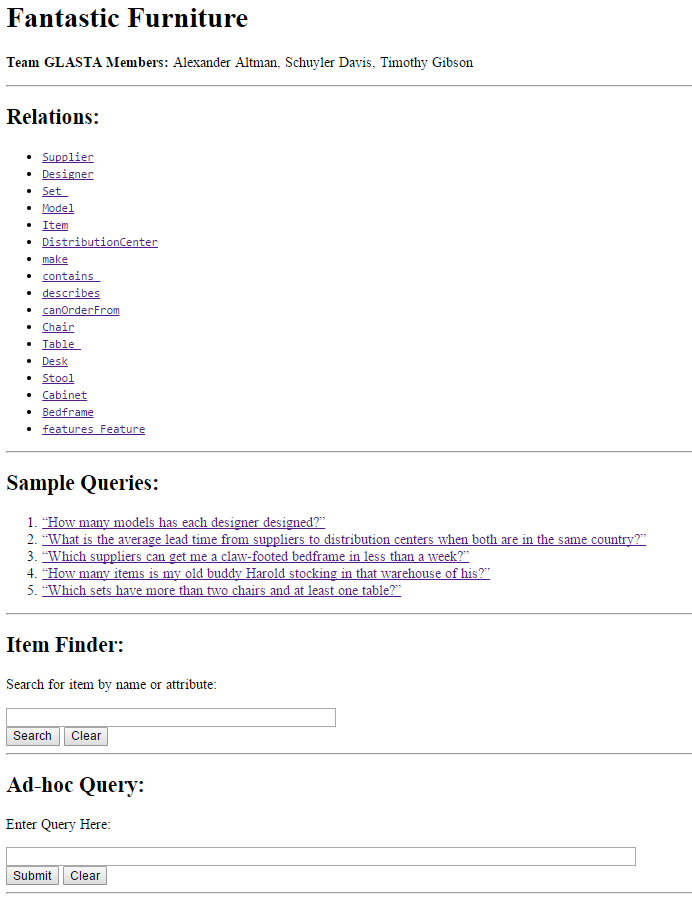
\includegraphics[keepaspectratio=true,width=40em,height=40em]{snapshots/frontpage.png}\\
\hline
\textbf{Relation View}\\*
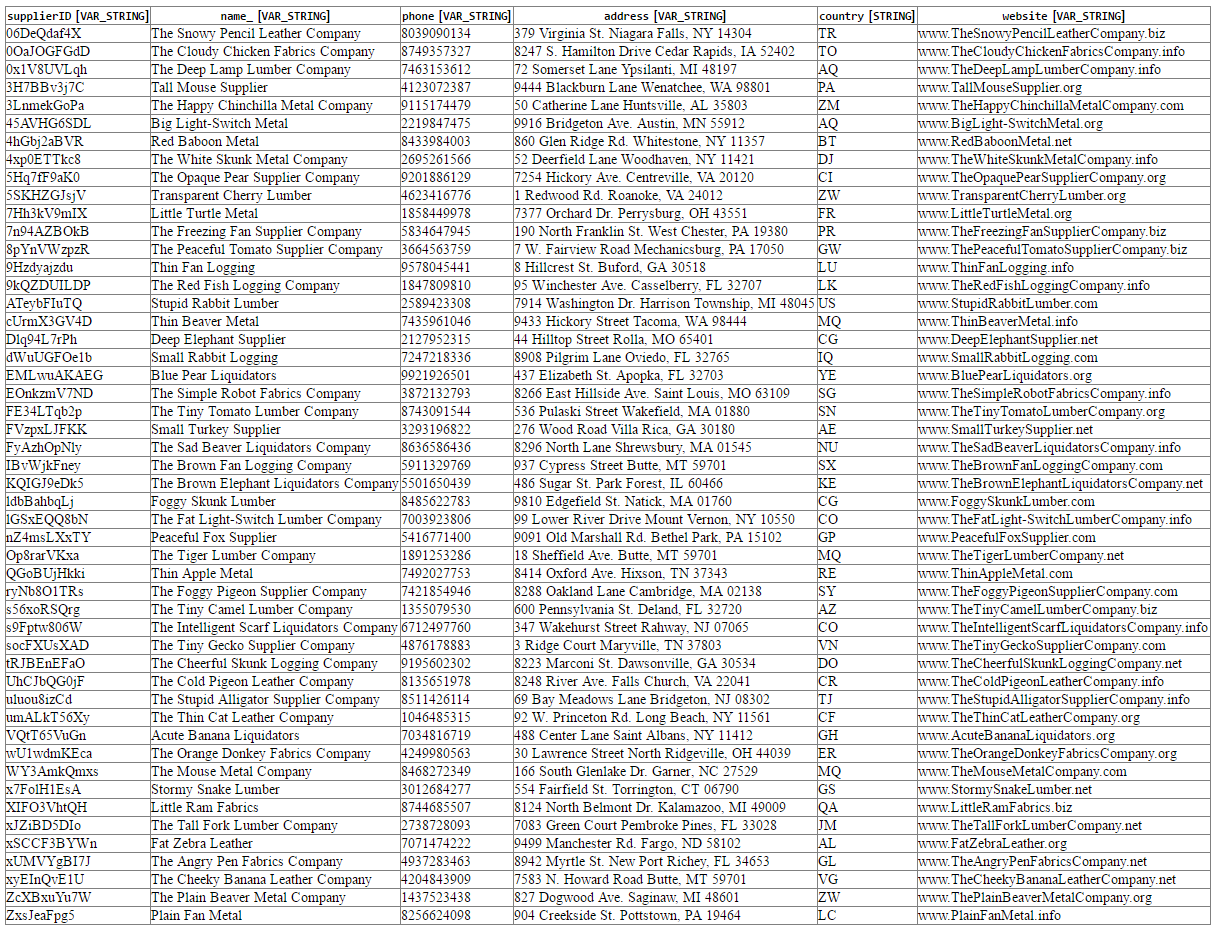
\includegraphics[keepaspectratio=true,width=40em,height=40em]{snapshots/sampleRelation.png}\\
\hline
\textbf{Sample Query}\\*
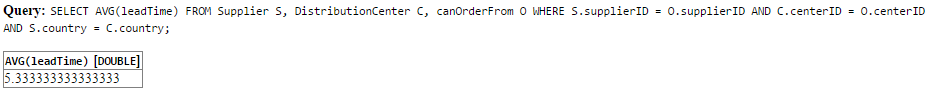
\includegraphics[keepaspectratio=true,width=40em,height=40em]{snapshots/sampleQuery.png}\\
\hline
\textbf{Search Query}\\*
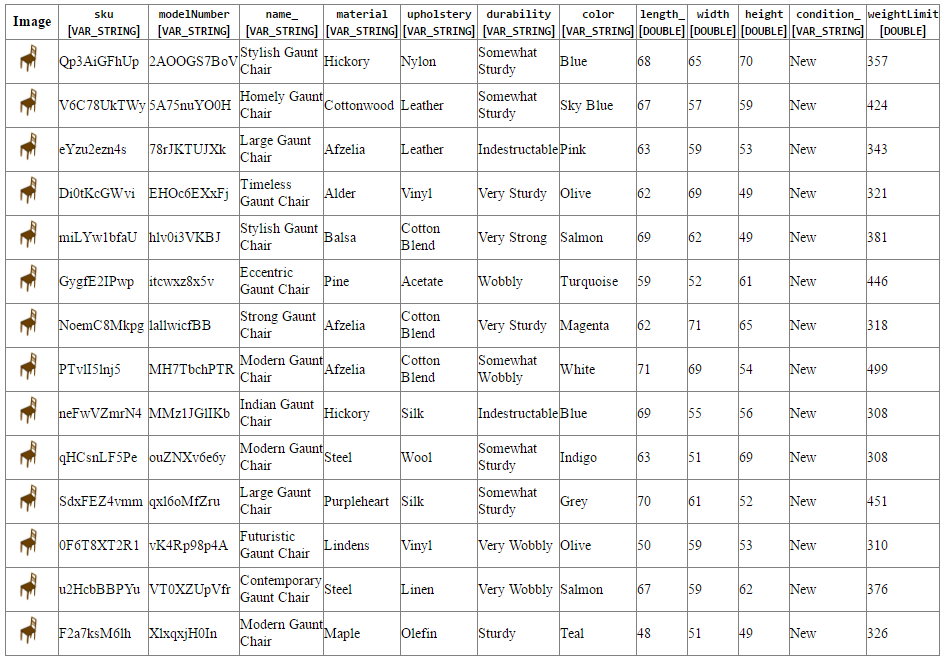
\includegraphics[keepaspectratio=true,width=40em,height=40em]{snapshots/sampleSearch.PNG}\\
\hline
\textbf{Ad\hyp Hoc Query}\\*
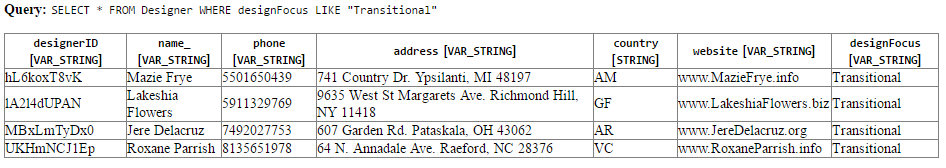
\includegraphics[keepaspectratio=true,width=40em,height=40em]{snapshots/sampleAdHoc.PNG}\\
\lasthline
\end{longtabu}

\backmatter
\section{Group Work}
\begin{samepage}%
\begin{enumerate}[leftmargin=*,widest={Alexander:}]

\item[Timothy:]
Timothy was the second draft coder, scripter, and art director.
Timothy checked Alexander's work, making sure the database implementation was coherent.
Timothy also wrote the bulk of the scripts that generated the data for the database.
Timothy also worked alongside Alexander in making sure the implementation was on task.
Finally, Timothy produced any non\hyp code, non\hyp diagrammatic assets that the various project stages needed.

\item[Alexander:]
Alexander was the dedicated first draft coder for all project parts.
He made sure that the basic framework of the database was always at least minimally functional, and had some input on later design stages as well.

\item[Schuyler:]
Schuyler filled the role of supervisory and conceptualizing.
Schuyler was in charge of stepping back and examining project implementation from different angles.
He also ensured things \textquote[][]{made sense} for our data domain.
He filled a mostly \textquote[][]{administrative} role.

\end{enumerate}%
\end{samepage}

\chapter{\emph{Appendix}: Website Source Code and Resources}

\section{Source Code}

Note that the contents of the file \mintinline[breaklines,breakanywhere]{text}{info.php} is not included here for security reasons; it contains only the definitions of the global variables \mintinline[breaklines,breakanywhere]{html+php}{username} and \mintinline[breaklines,breakanywhere]{html+php}{passwork}.
The misspelling of the latter variable's name was not intentional, but it has been maintained anyway for backwards compatibility purposes.

\subsection{\texorpdfstring{\mintinline[breaklines,breakanywhere]{text}{index.php}}{\texttt{index.php}}}

\inputminted[linenos,breaklines,breakanywhere]{html+php}{index.php}

\subsection{\texorpdfstring{\mintinline[breaklines,breakanywhere]{text}{conn.php}}{\texttt{conn.php}}}

\inputminted[linenos,breaklines,breakanywhere]{html+php}{conn.php}

\subsection{\texorpdfstring{\mintinline[breaklines,breakanywhere]{text}{relation.php}}{\texttt{relation.php}}}

\inputminted[linenos,breaklines,breakanywhere]{html+php}{relation.php}

\subsection{\texorpdfstring{\mintinline[breaklines,breakanywhere]{text}{finder.php}}{\texttt{finder.php}}}

\inputminted[linenos,breaklines,breakanywhere]{html+php}{finder.php}

\subsection{\texorpdfstring{\mintinline[breaklines,breakanywhere]{text}{query.php}}{\texttt{query.php}}}

\inputminted[linenos,breaklines,breakanywhere]{html+php}{query.php}

\section{Resources}

\subsection{\texorpdfstring{\mintinline[breaklines,breakanywhere]{text}{chair.png}}{\texttt{chair.png}}}

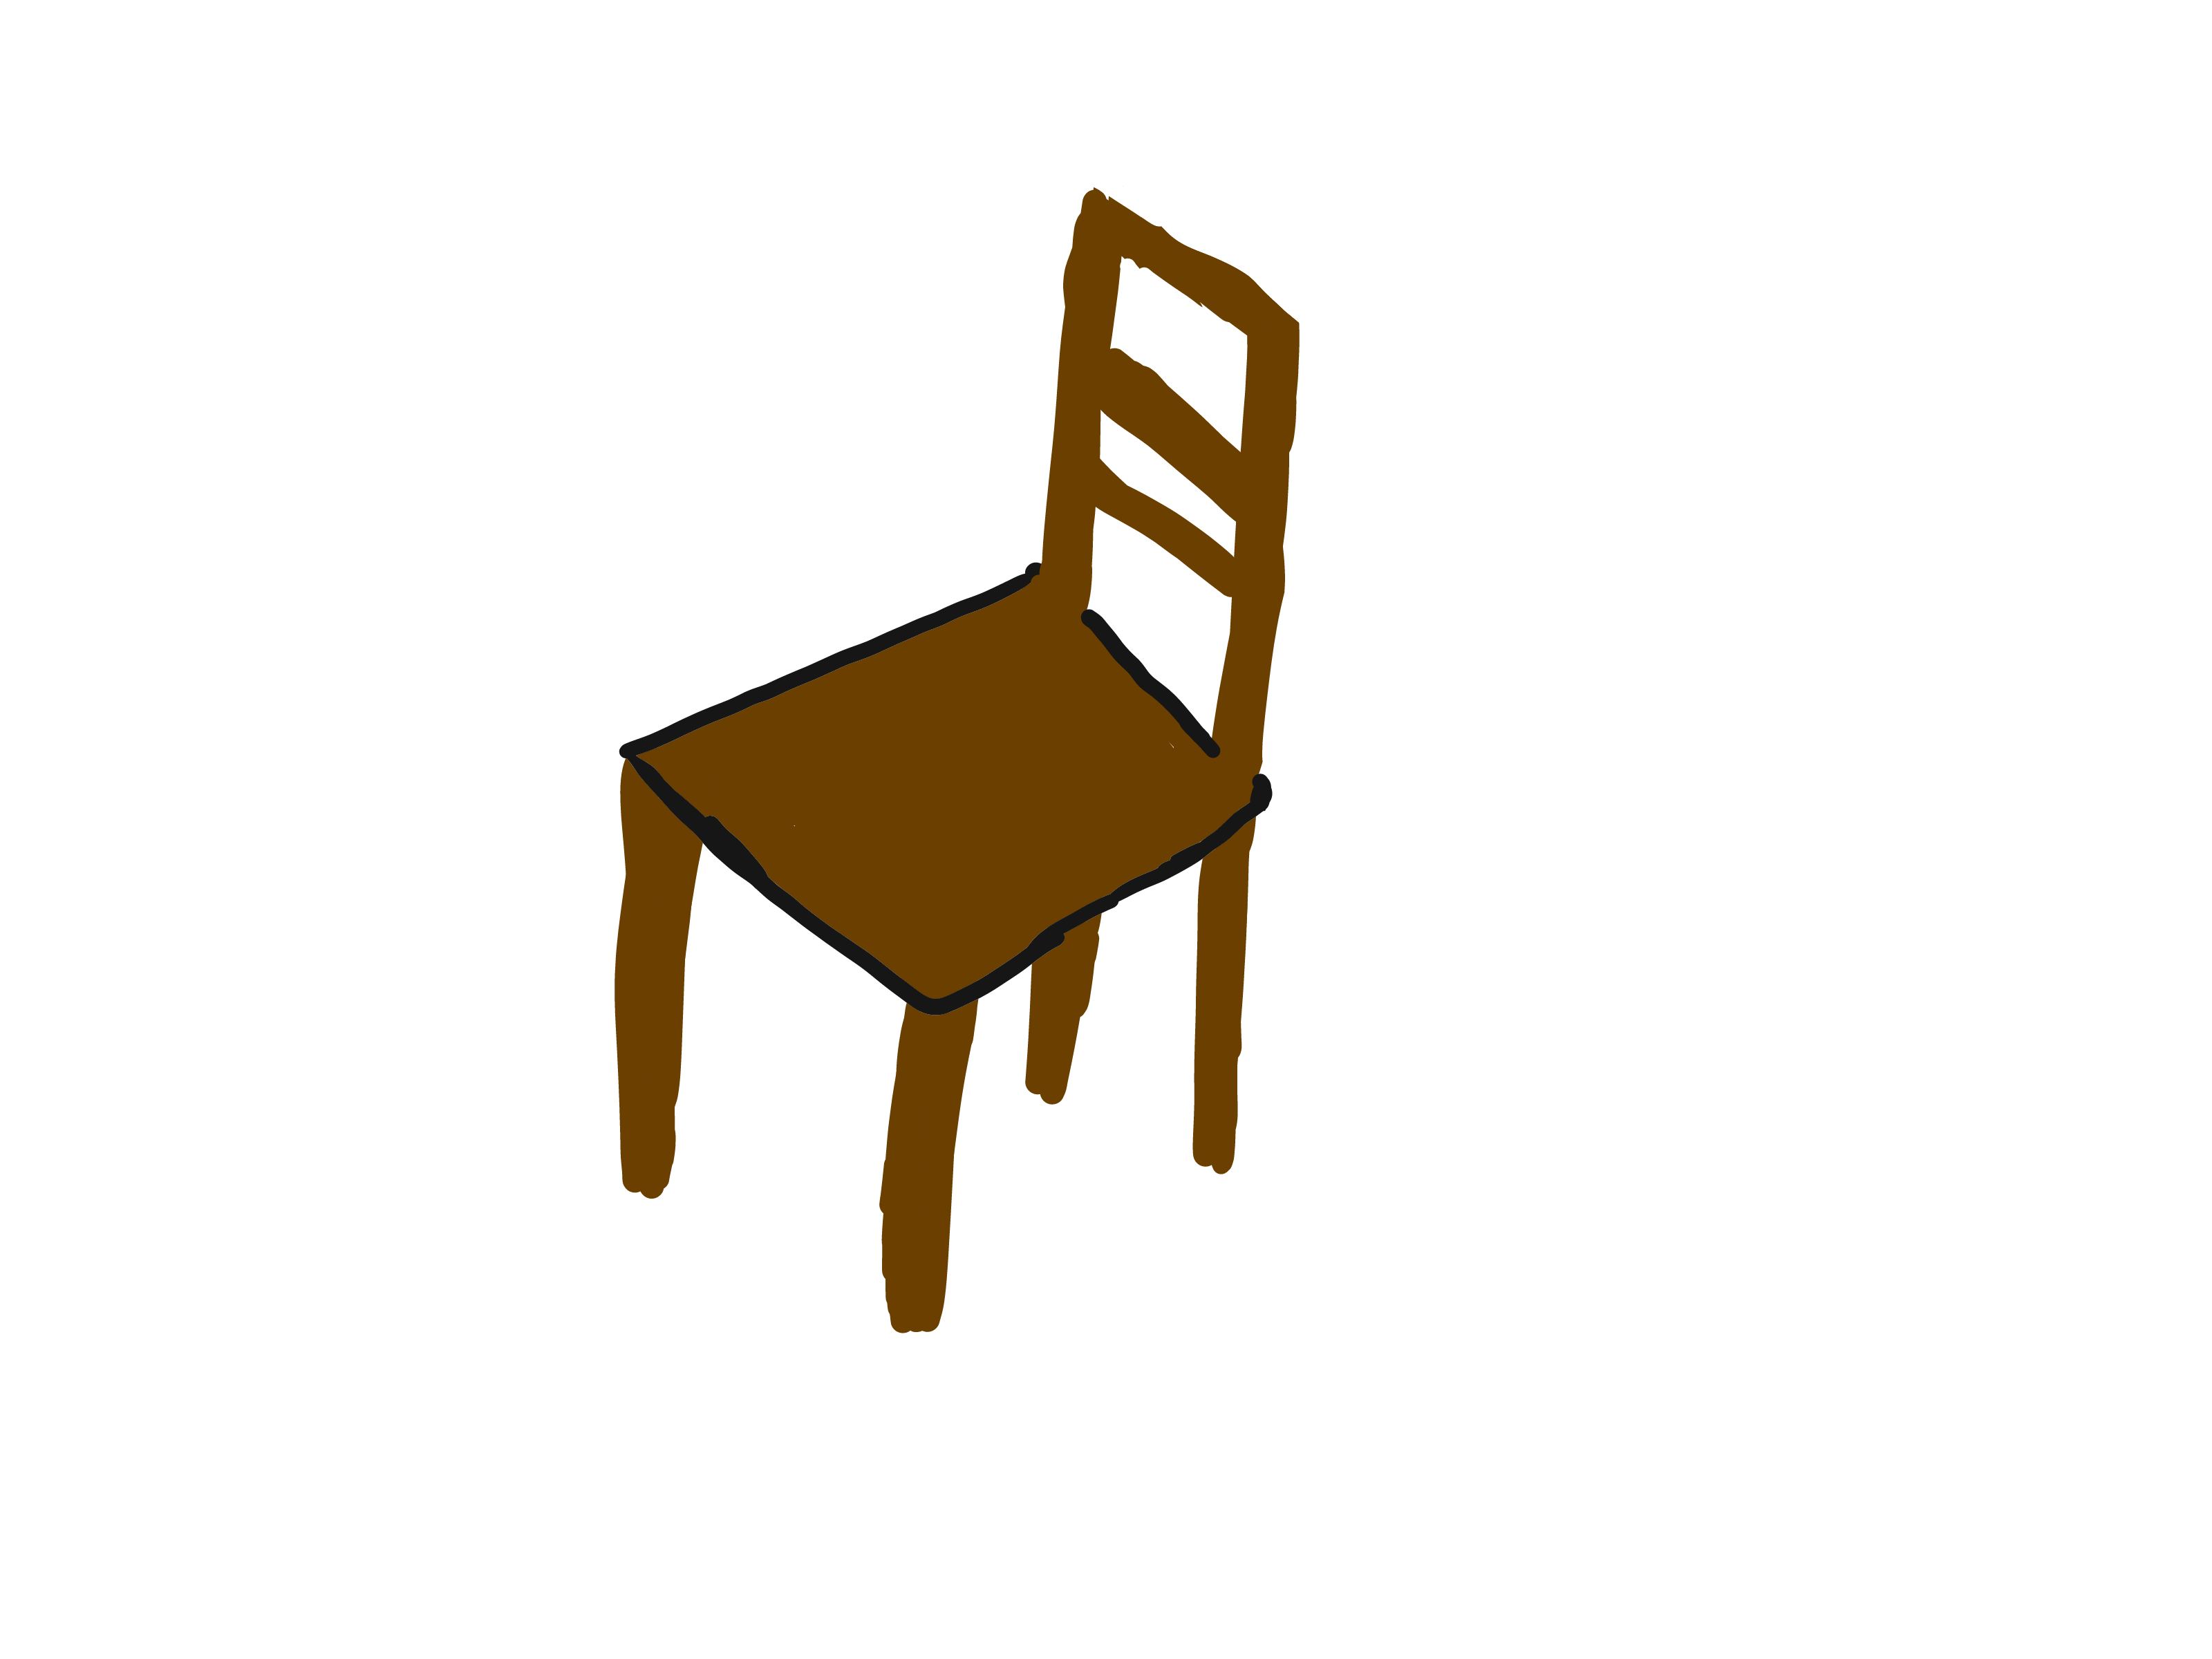
\includegraphics[keepaspectratio=true,width=20em,height=20em]{product_Images/chair.png}

\subsection{\texorpdfstring{\mintinline[breaklines,breakanywhere]{text}{cabinet.png}}{\texttt{cabinet.png}}}

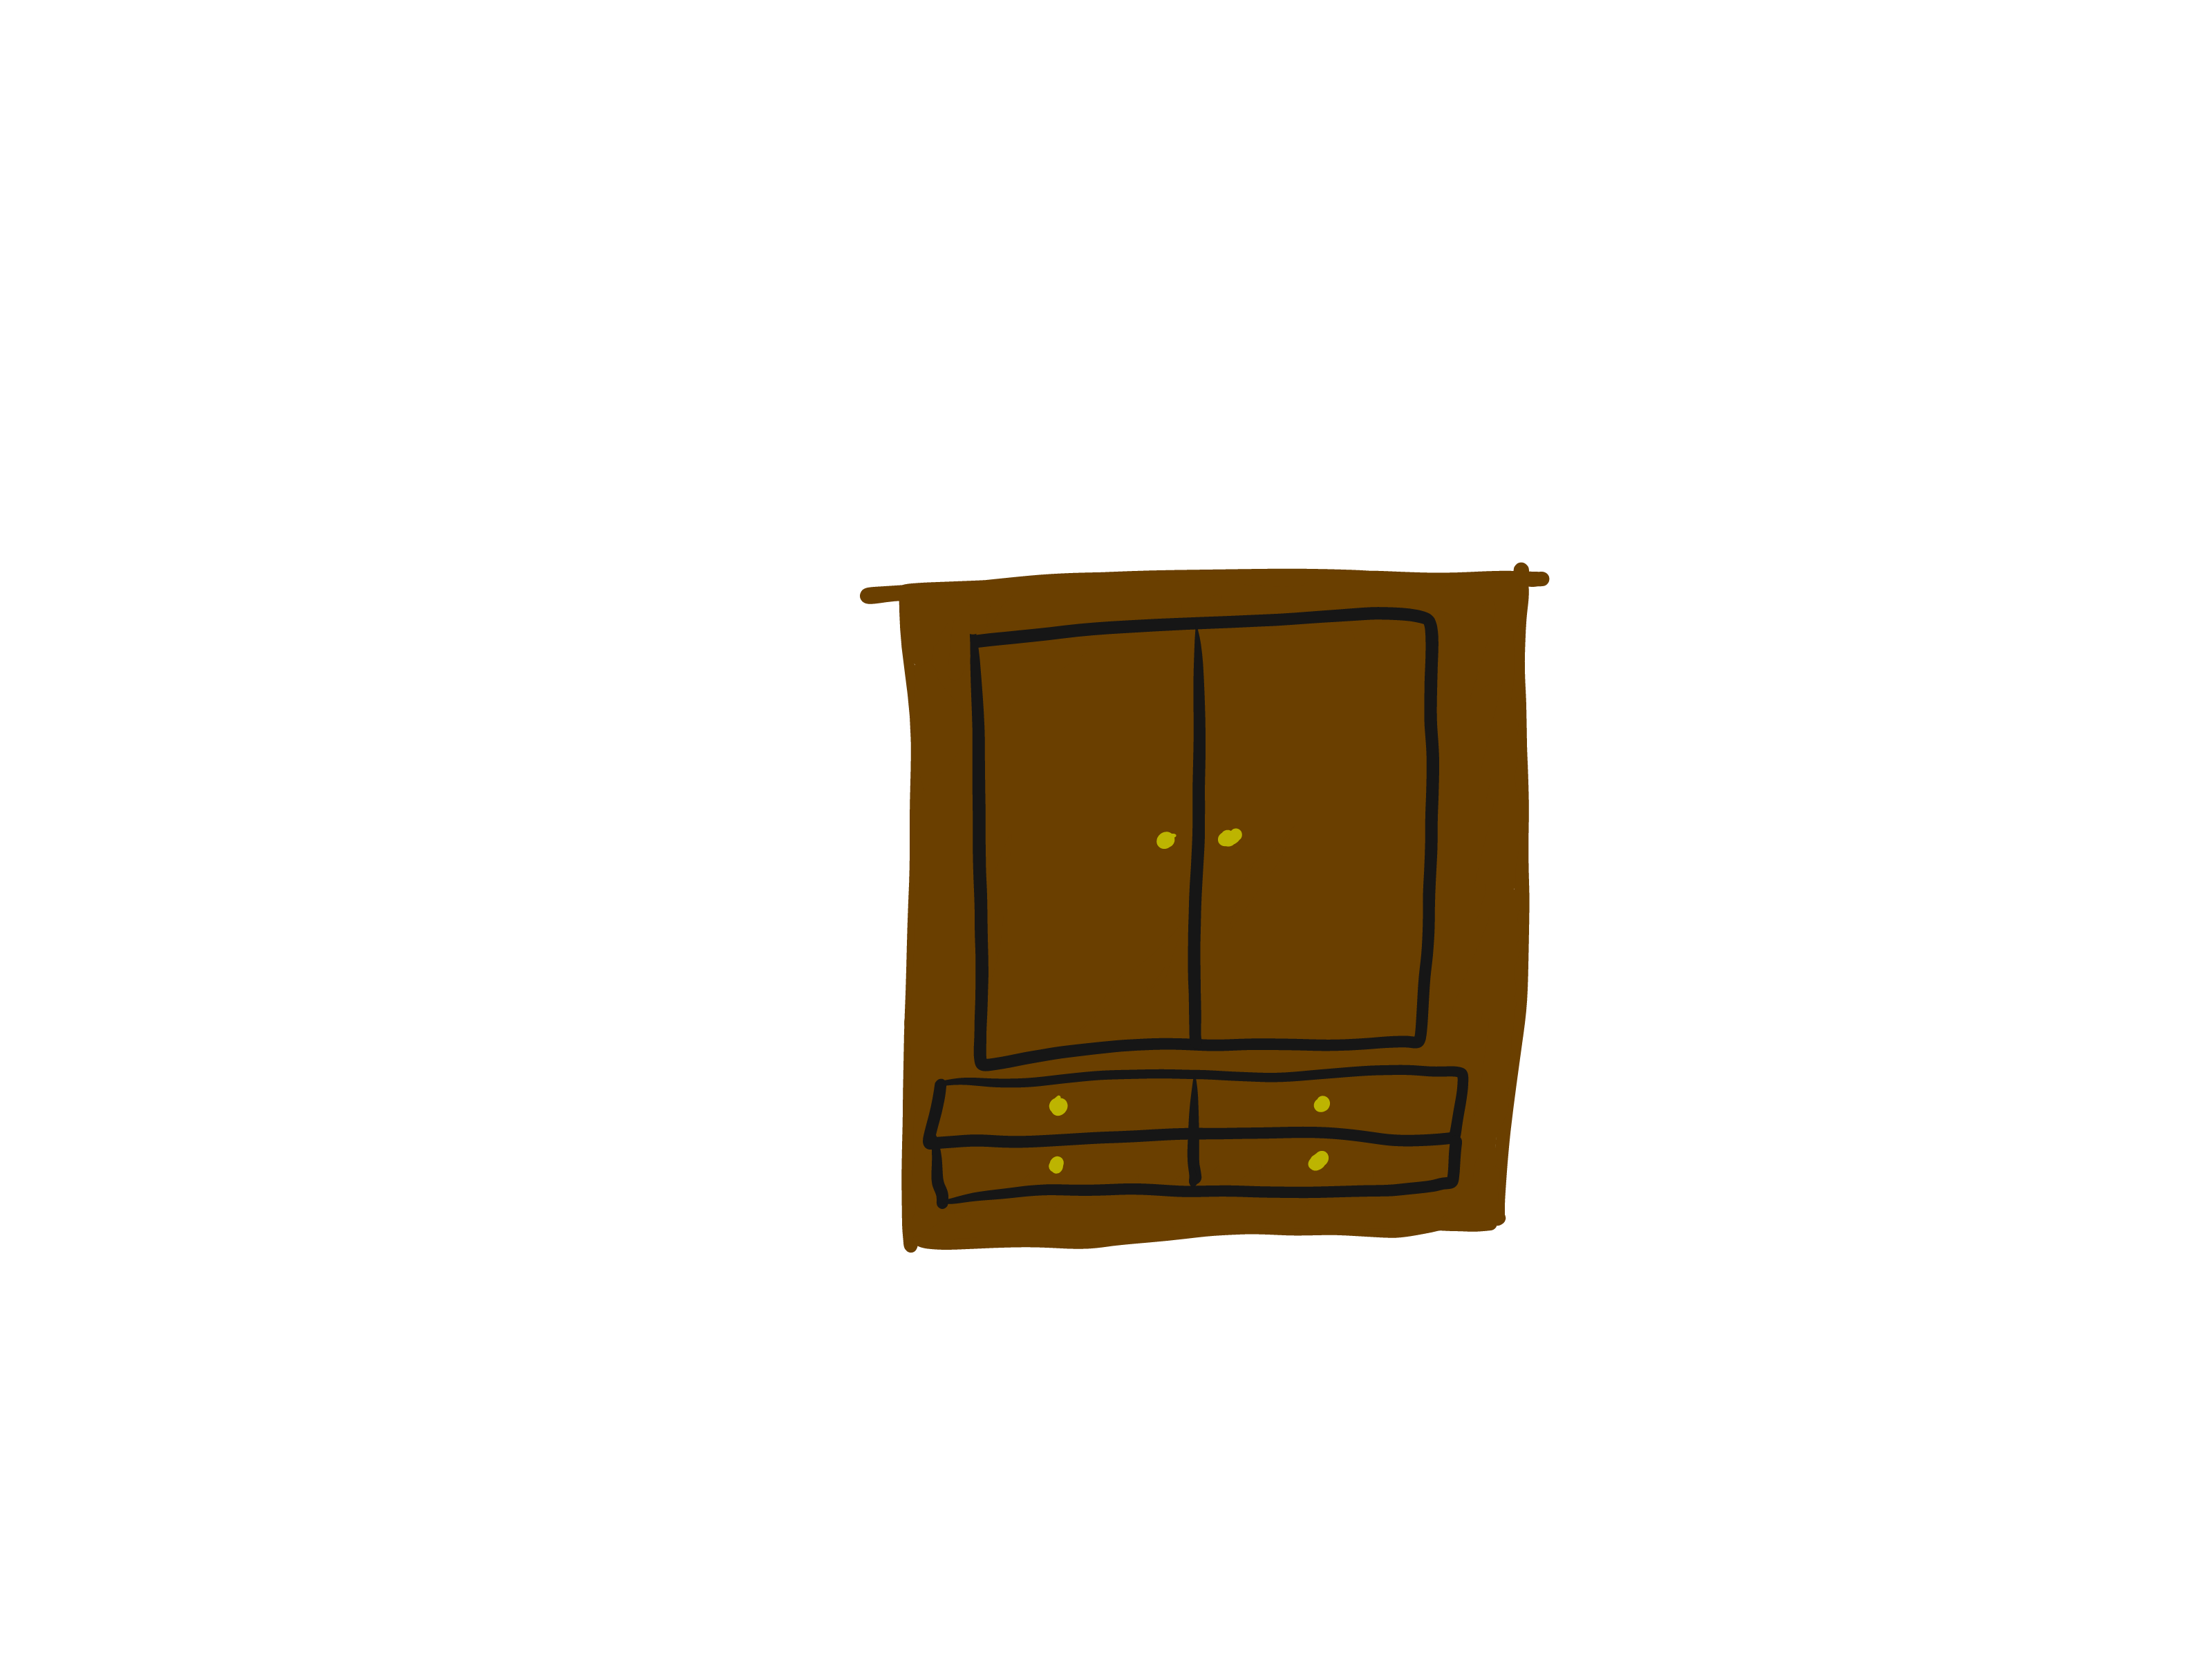
\includegraphics[keepaspectratio=true,width=20em,height=20em]{product_Images/cabinet.png}

\subsection{\texorpdfstring{\mintinline[breaklines,breakanywhere]{text}{desk.png}}{\texttt{desk.png}}}

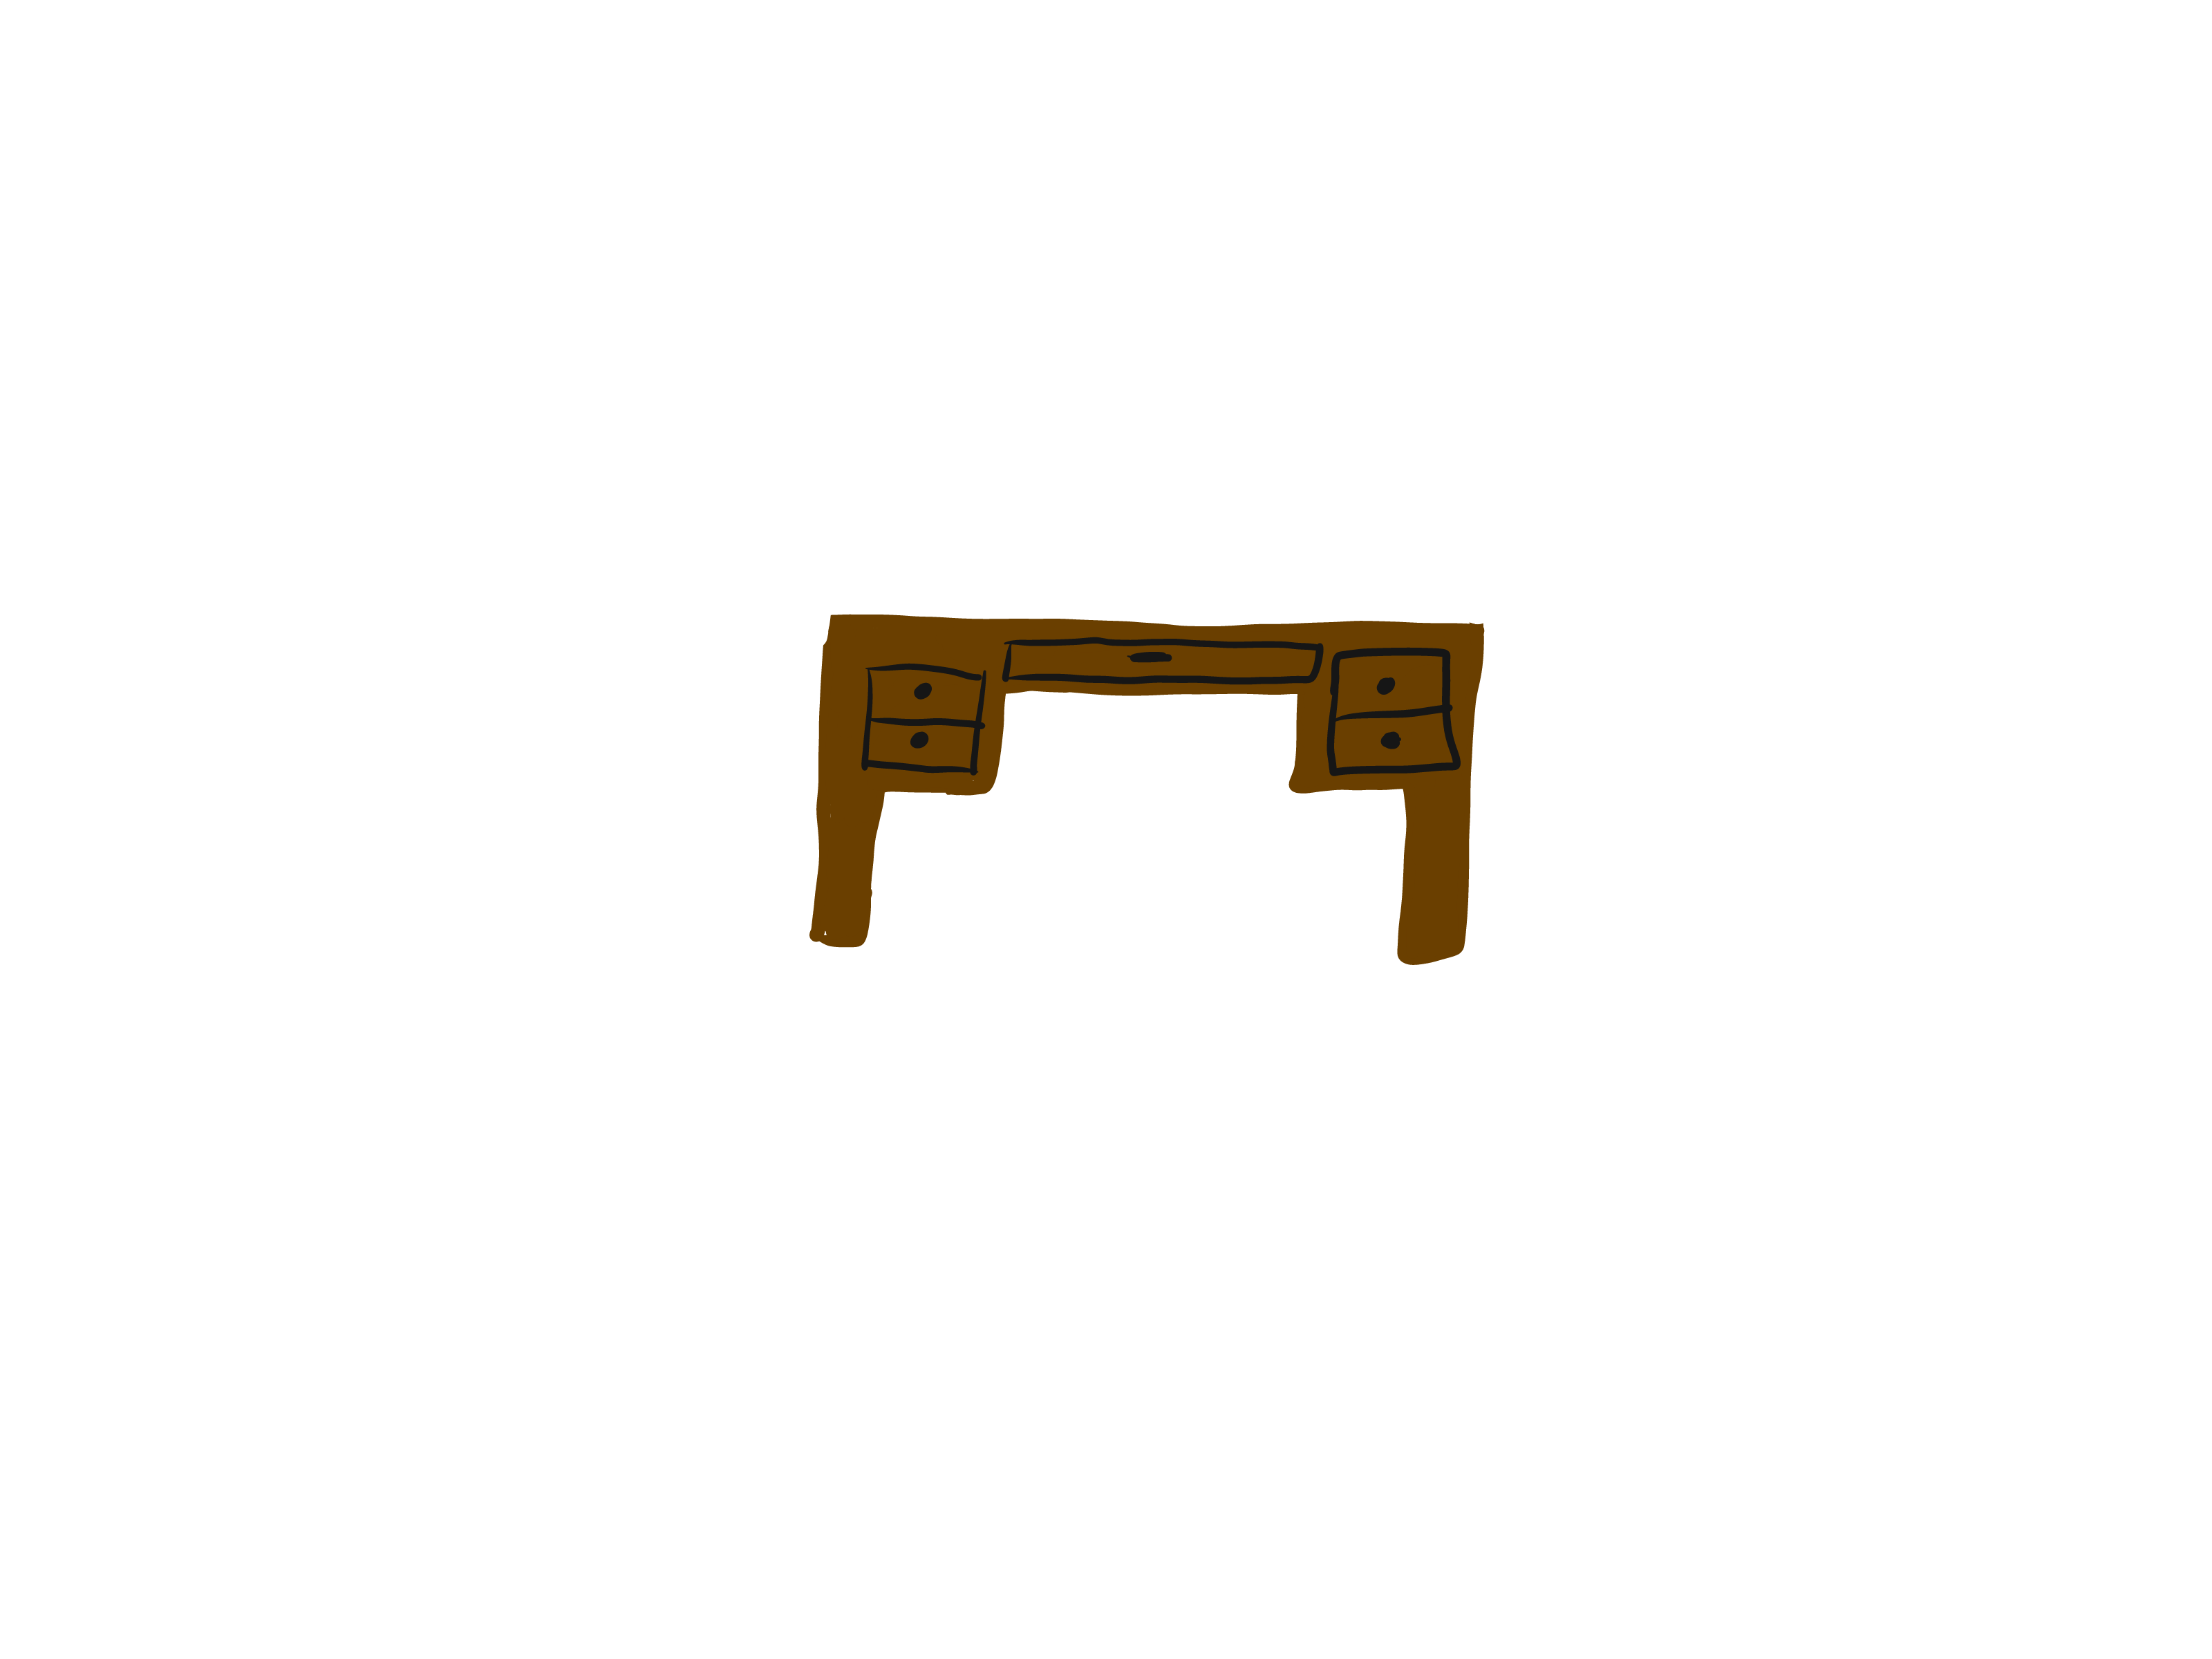
\includegraphics[keepaspectratio=true,width=20em,height=20em]{product_Images/desk.png}

\subsection{\texorpdfstring{\mintinline[breaklines,breakanywhere]{text}{bedframe.png}}{\texttt{bedframe.png}}}

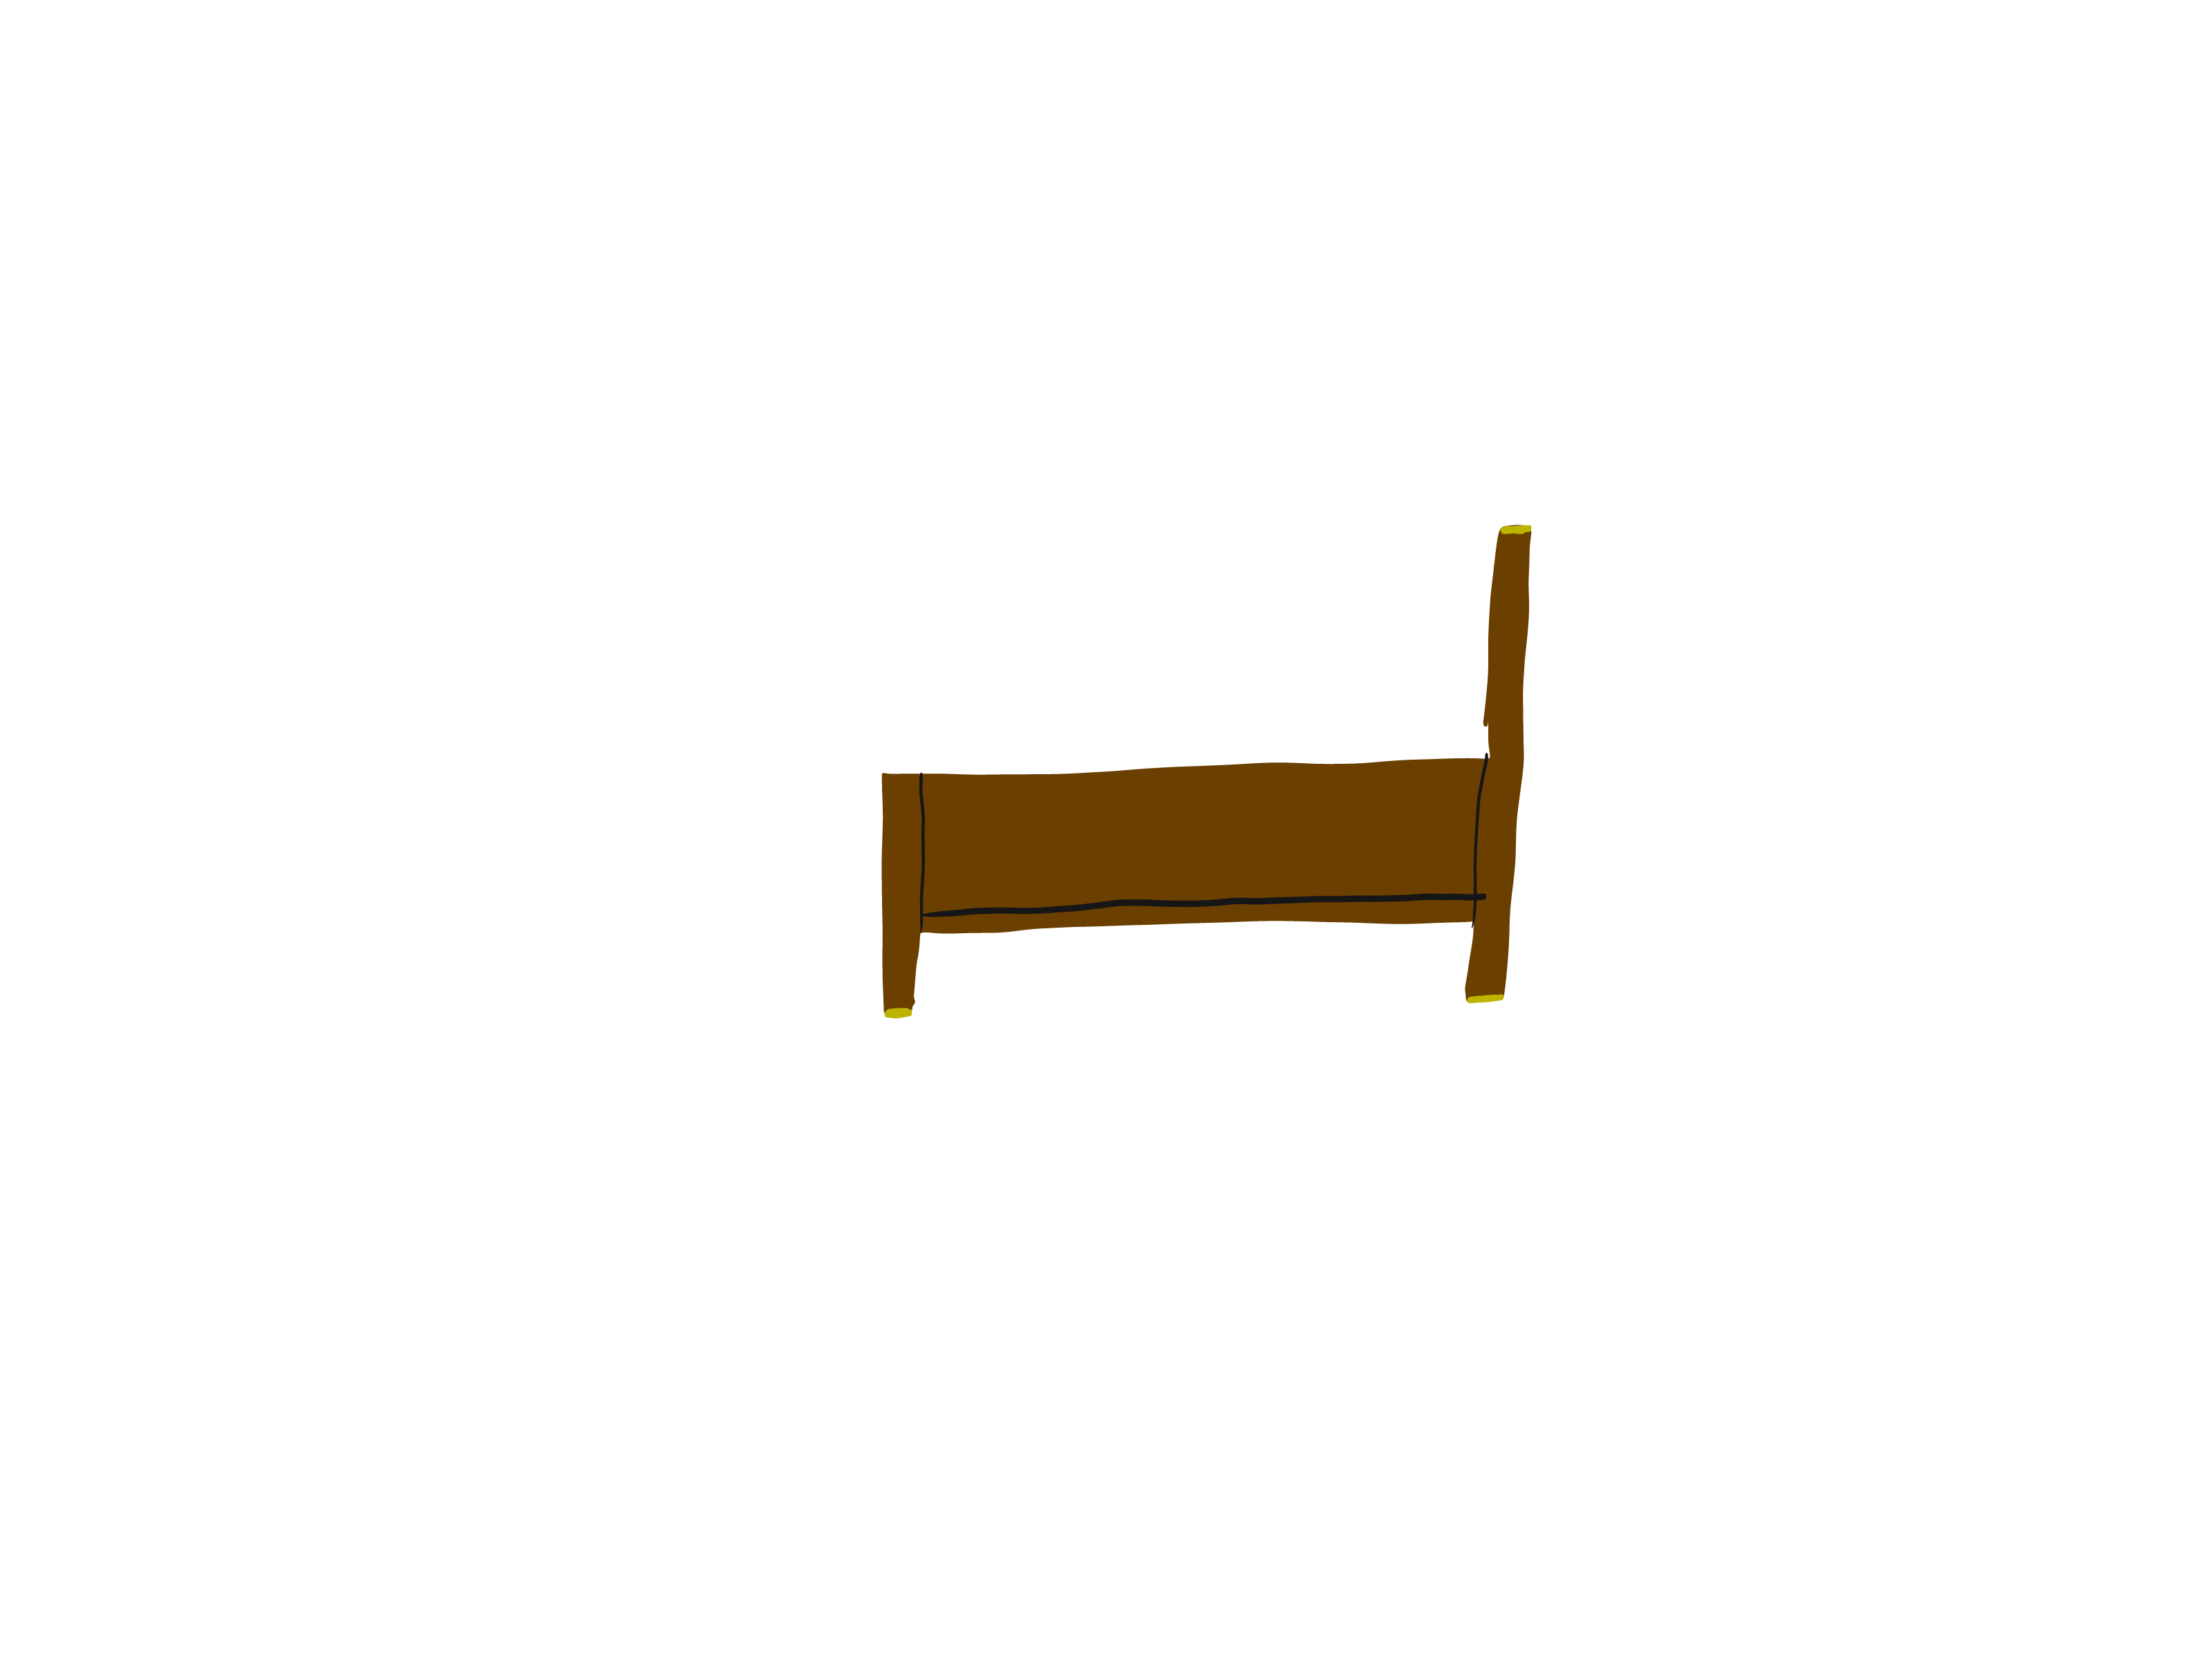
\includegraphics[keepaspectratio=true,width=20em,height=20em]{product_Images/bedframe.png}

\subsection{\texorpdfstring{\mintinline[breaklines,breakanywhere]{text}{stool.png}}{\texttt{stool.png}}}

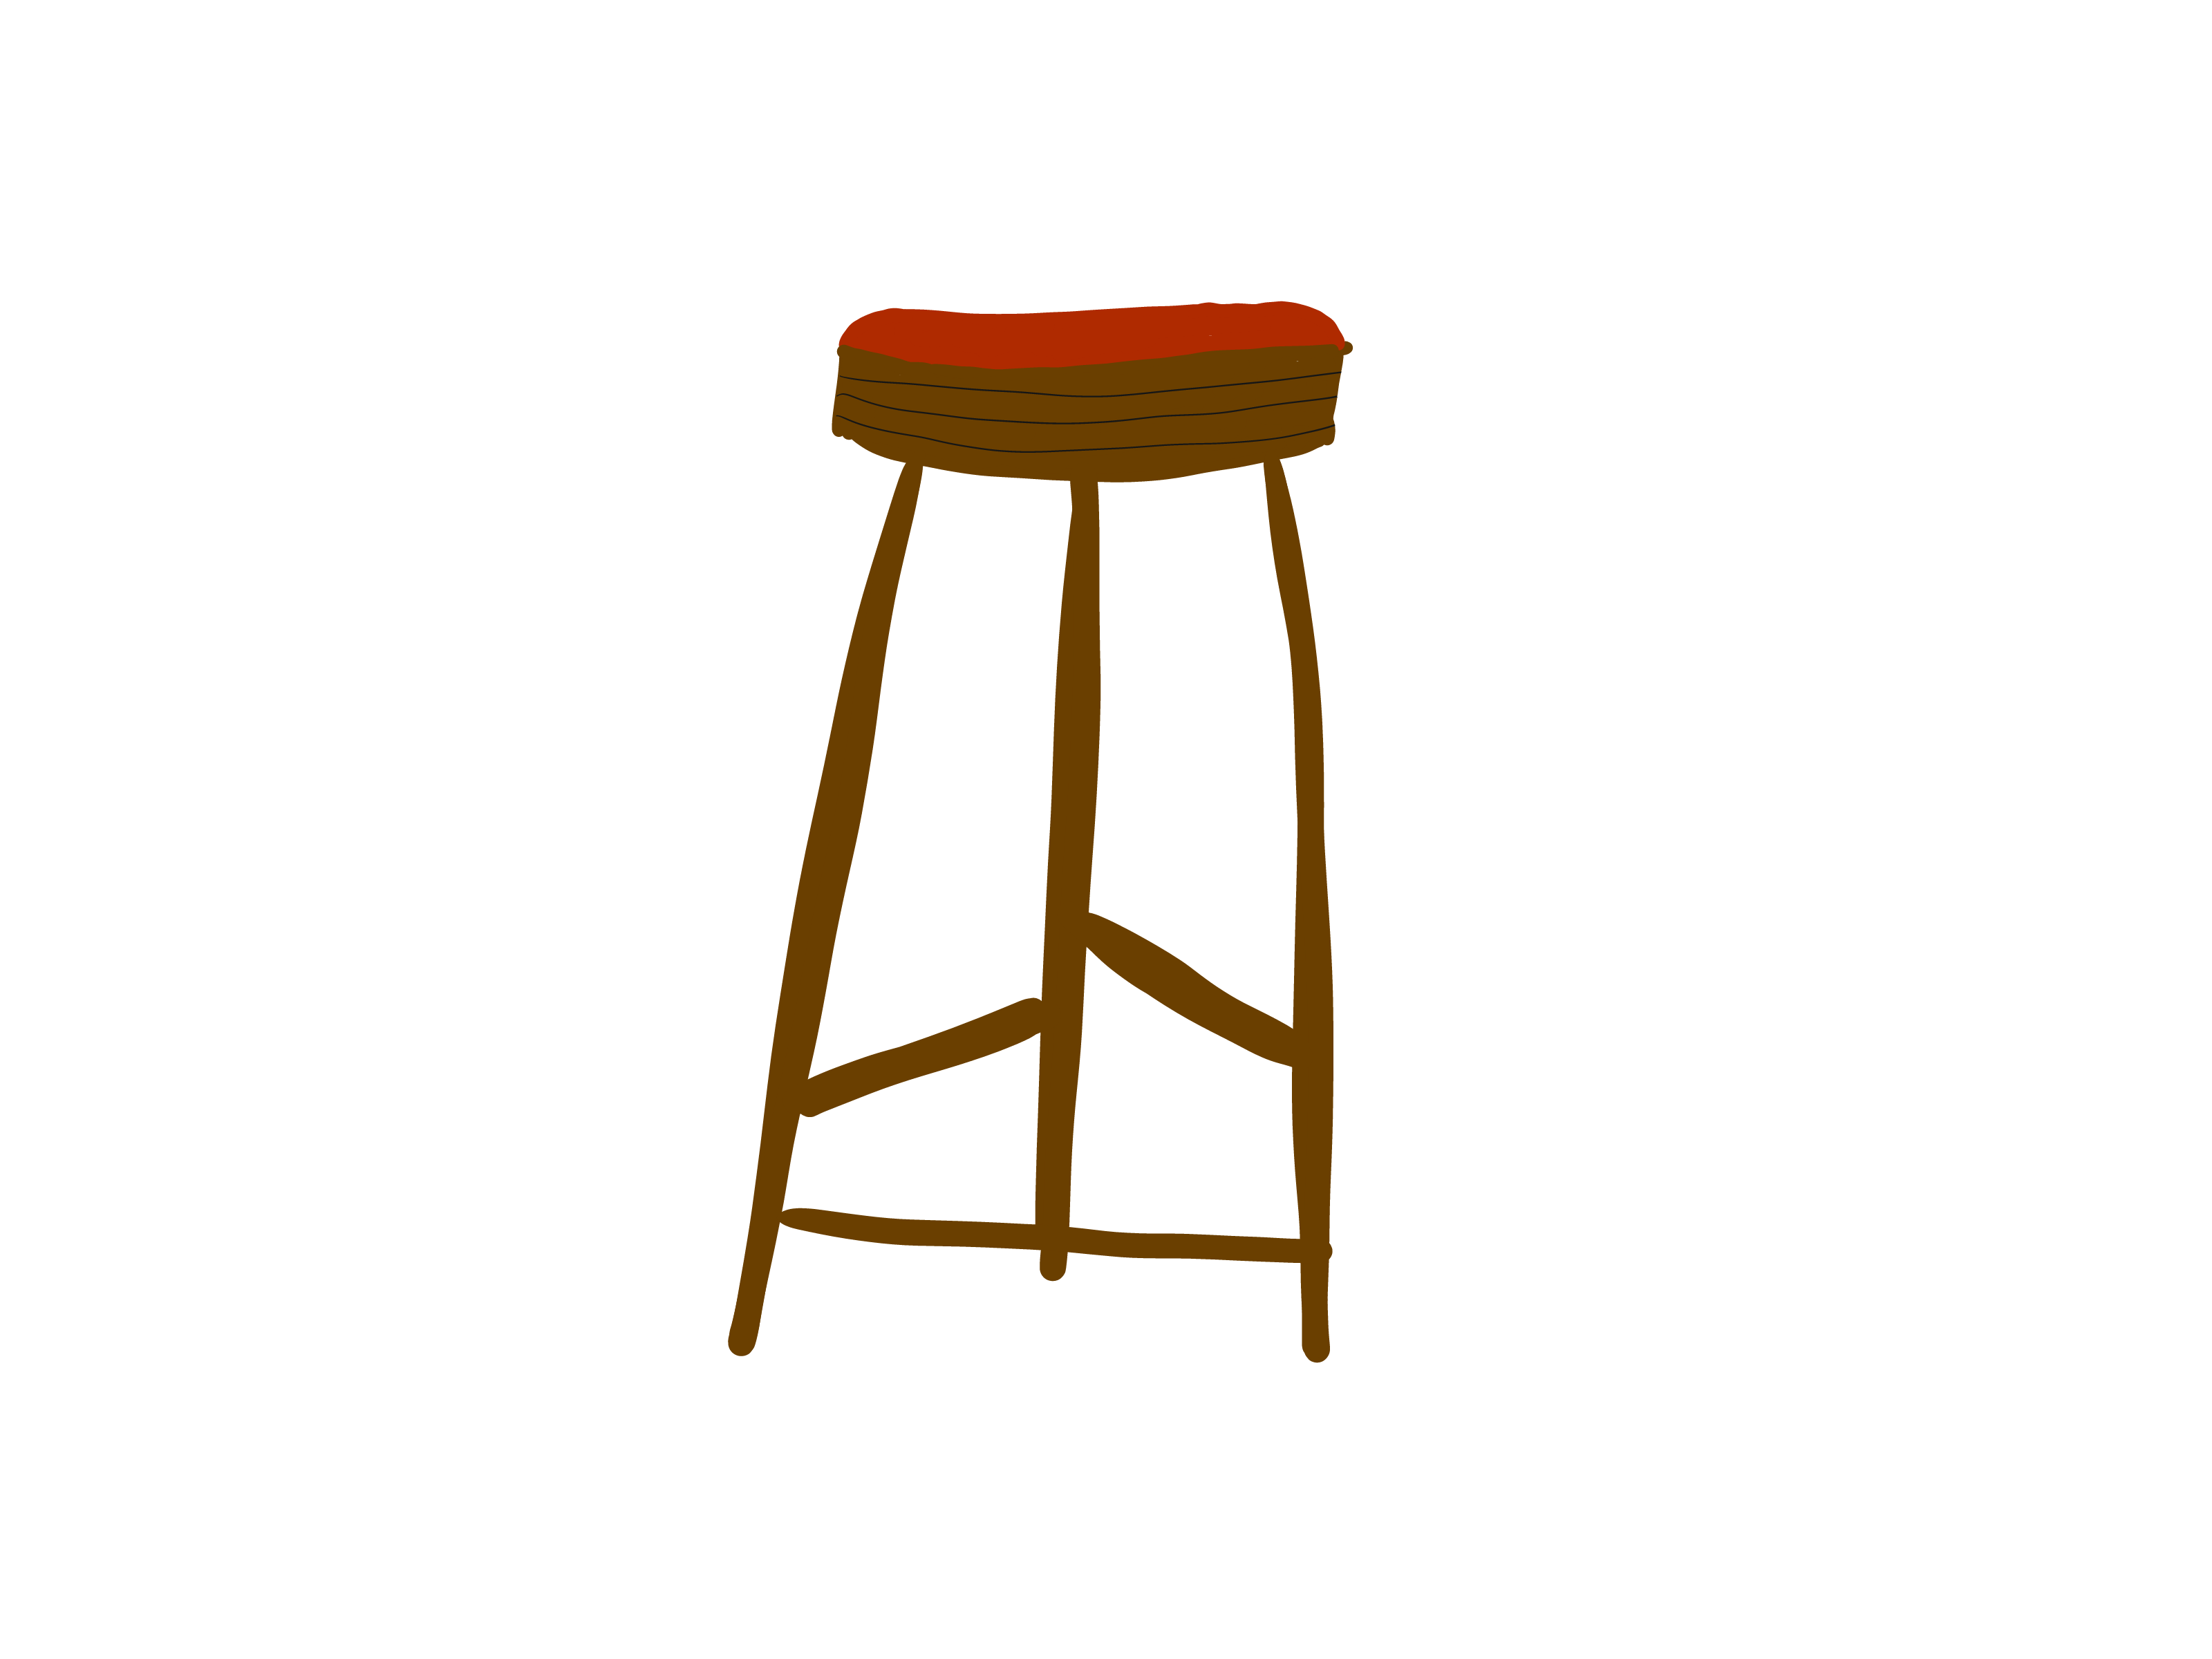
\includegraphics[keepaspectratio=true,width=20em,height=20em]{product_Images/stool.png}

\subsection{\texorpdfstring{\mintinline[breaklines,breakanywhere]{text}{table.png}}{\texttt{table.png}}}

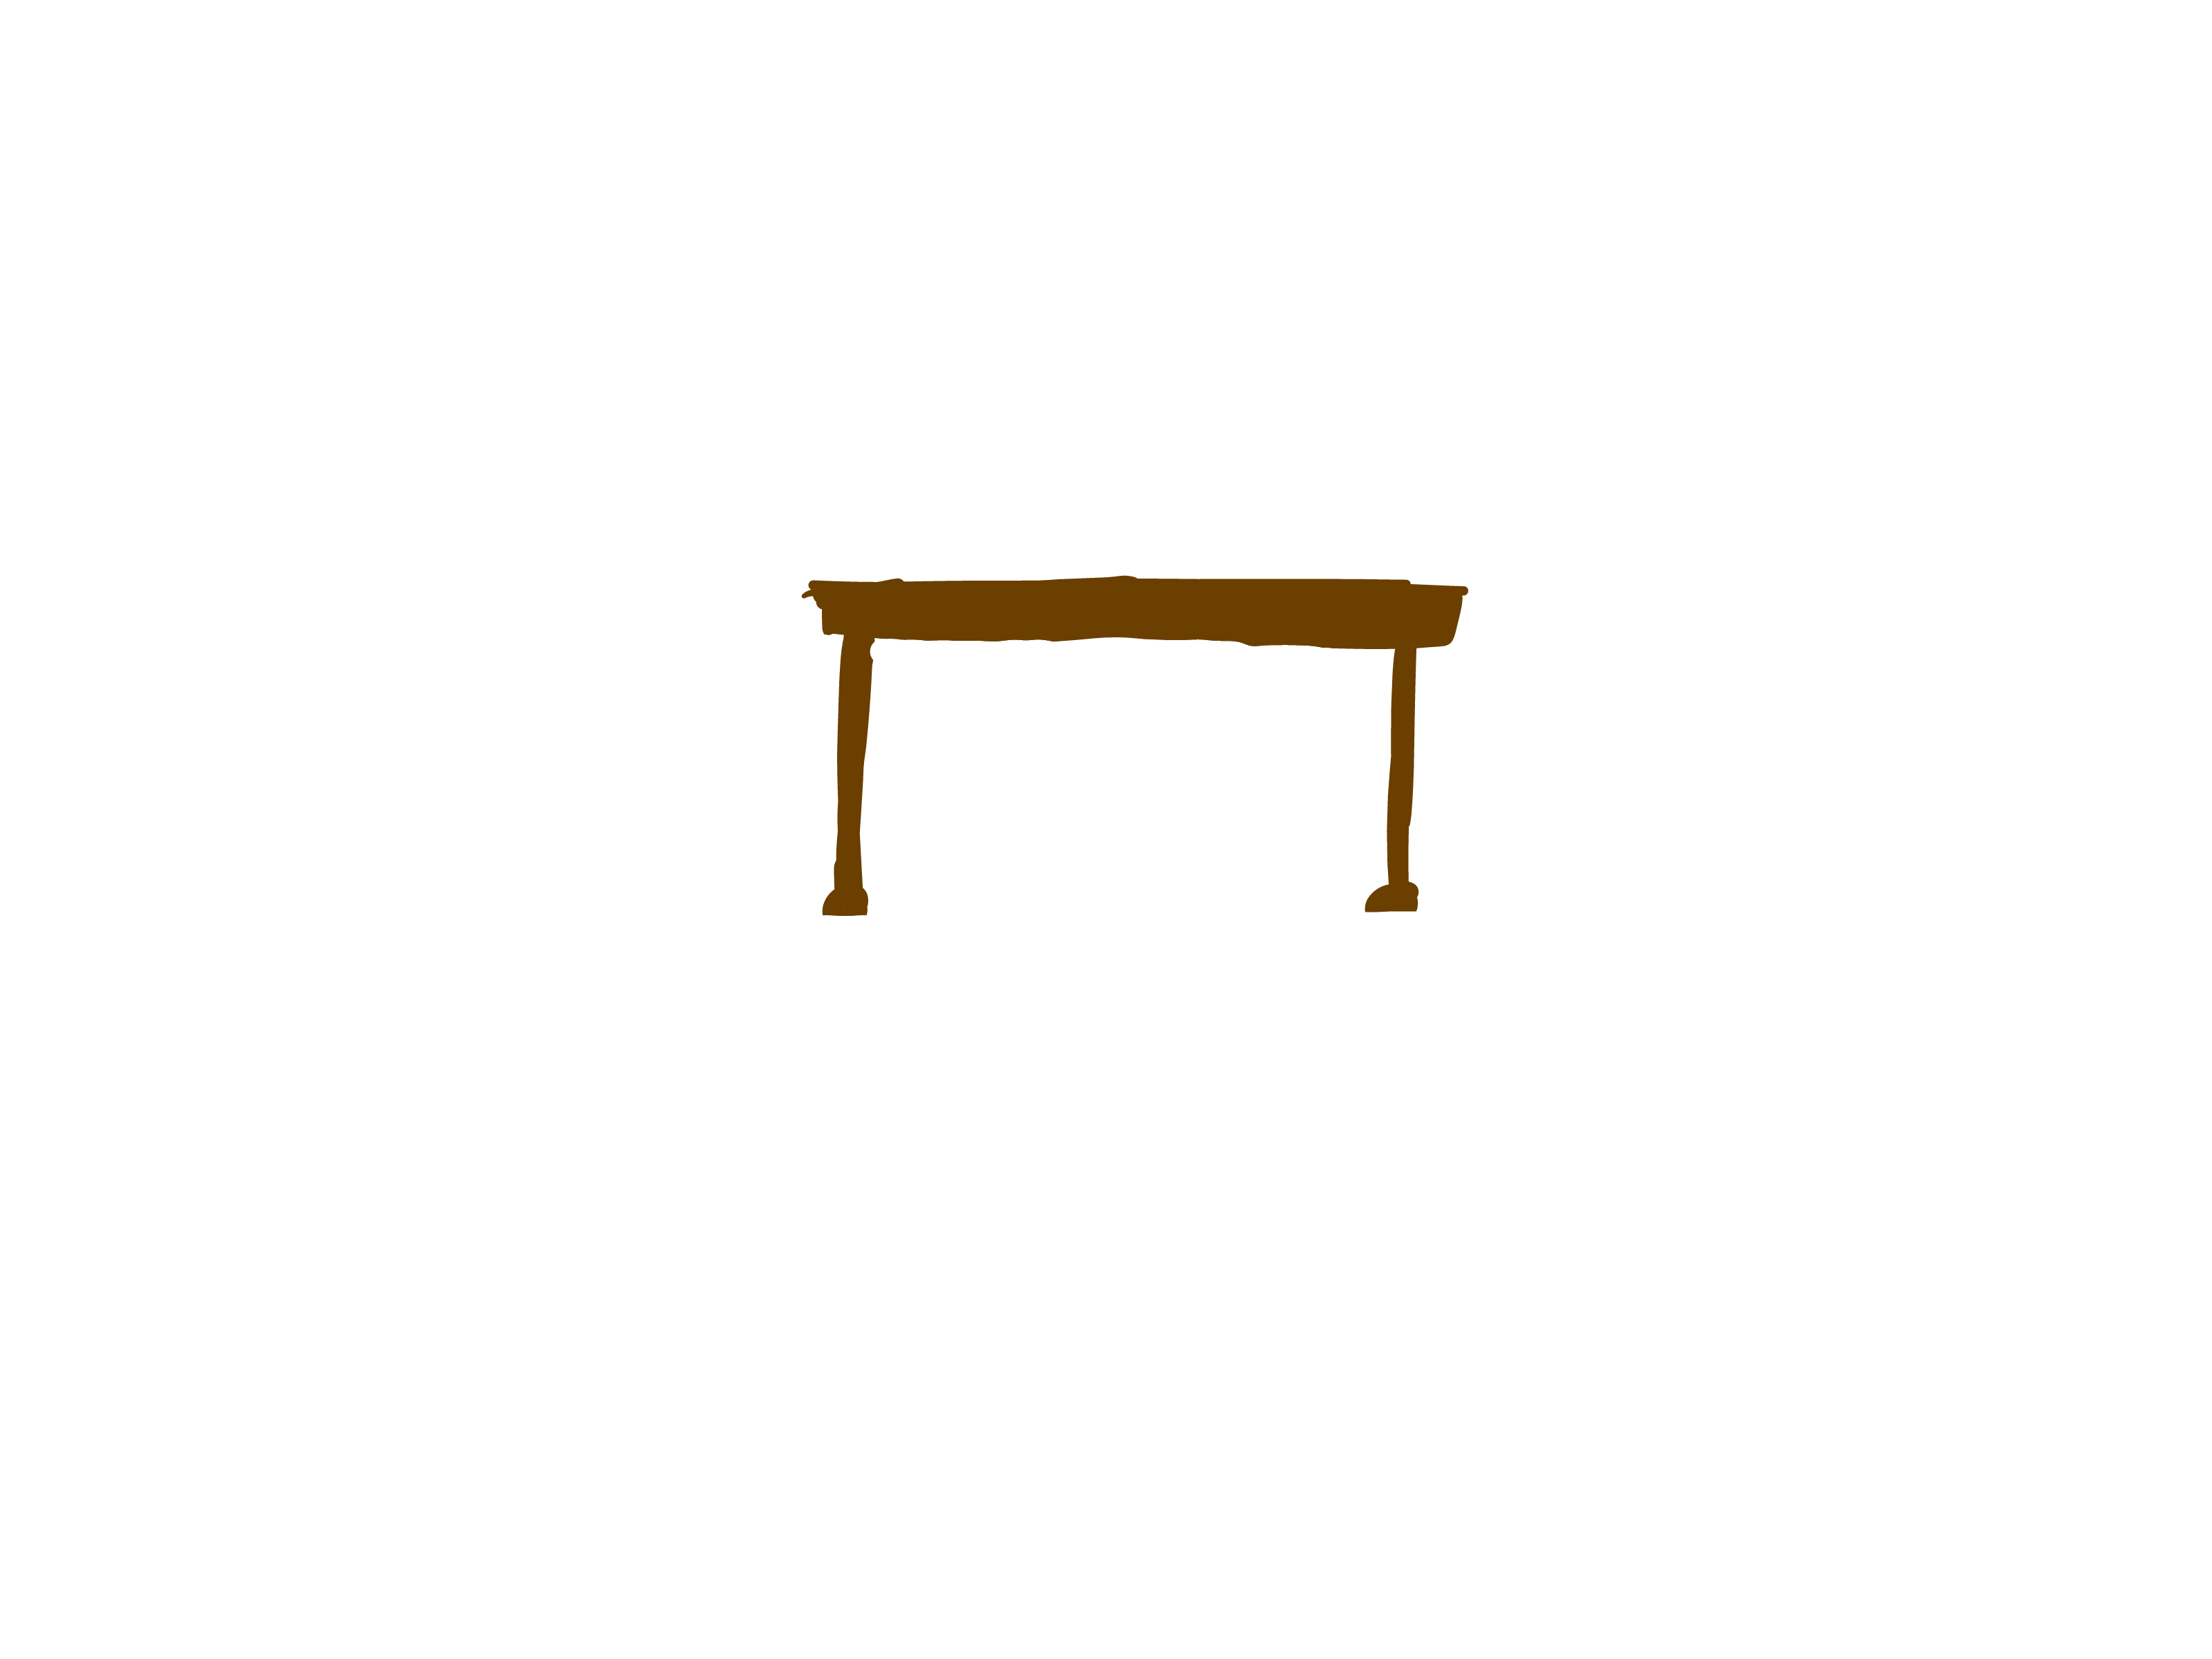
\includegraphics[keepaspectratio=true,width=20em,height=20em]{product_Images/table.png}

\end{document}
